% template file include
% A4 lap méret, 12 pontos betűméret
\documentclass[12pt,a4paper]{article}

% szükséges csomagok
\usepackage[utf8]{inputenc}
\usepackage[T1]{fontenc}
\usepackage[english]{babel}
\usepackage{float}
\usepackage{graphicx}
\usepackage{pdfpages}
\usepackage{caption}
\usepackage[colorlinks=false, pdfborder={0 0 0}, linkcolor=black, unicode]{hyperref}
\usepackage{mathtools}
\usepackage{relsize}
\usepackage{amsmath}
\usepackage{amsfonts}
\usepackage{amssymb}
\usepackage{listings}
\usepackage{csquotes}
\usepackage{enumitem}
\usepackage{url}
\usepackage[nottoc,numbib]{tocbibind}
\usepackage{titlesec}
\usepackage{titletoc}
\usepackage{tabularx}

% lista elemek közti hely, és vonal mint lista elem előtti jel beállítása
\setlist{nosep, label={--}}

% tartalomjegyzék formázása
\dottedcontents{section}[1.5em]{}{1.5em}{1pc}
\dottedcontents{subsection}[3em]{}{2em}{1pc}
\dottedcontents{subsubsection}[5em]{}{3em}{1pc}

% fejezet cím formázás: 14 pontos betűméret, nagybetűs
\titleformat{\section}{\normalfont\fontsize{14}{14}\mdseries\MakeUppercase}{\thesection}{1em}{}
\titleformat{\subsection}{\normalfont\fontsize{12}{12}\bfseries}{\thesubsection}{1em}{}
\titleformat{\subsubsection}{\normalfont\fontsize{12}{12}\bfseries}{\thesubsubsection}{1em}{}

% fejezet cím térközök
\titlespacing*{\section}{0em}{0em}{1em}
\titlespacing*{\subsection}{0em}{1em}{1em}
\titlespacing*{\subsubsection}{0em}{1em}{1em}


% margó
\usepackage[right=2.50cm, 
            left=3.50cm, 
            top=2.50cm, 
            bottom=4.00cm
            ]{geometry}

% sorköz
\linespread{1.15}

% times new roman betűtípus
\usepackage{times}

% ábra és táblázat számozás beállítása fejezetenként
\setcounter{figure}{0}
\renewcommand{\thefigure}{\arabic{section}.\arabic{figure}}
\setcounter{table}{0}
\renewcommand{\thetable}{\arabic{section}.\arabic{table}}
\numberwithin{equation}{section}
\numberwithin{figure}{section}

% ábra, táblázat cím formázás
\captionsetup[figure]{labelfont={it, small},textfont={it, small},labelsep=colon}
\captionsetup[table]{labelfont={it, small},textfont={it, small},labelsep=colon}

% hivatkozások formátuma és bib fájl importálása
\usepackage[backend=biber,style=ieee,doi=true,isbn=true,url=false,eprint=false]{biblatex}
\addbibresource{references.bib}

% bekezdés behúzása
\setlength{\parindent}{5 mm}

% bekezdés térköz
\setlength{\parskip}{8pt}

% ábra és táblajegyzék formázása
\makeatletter
\renewcommand\listoffigures{
    \section{\listfigurename}
      \@mkboth{\MakeUppercase\listfigurename}%
              {\MakeUppercase\listfigurename}%
    \@starttoc{lof}%
    }

\renewcommand\listoftables{
    \section{\listtablename}
      \@mkboth{\MakeUppercase\listtablename}%
              {\MakeUppercase\listtablename}%
    \@starttoc{lot}%
    }
\makeatother


\usepackage{listings}
\usepackage{xcolor}
\usepackage{algorithm}
\usepackage{algorithmicx}
\usepackage{algpseudocode}

\lstdefinestyle{sharpc}{language=[Sharp]C, frame=lr, rulecolor=\color{blue!80!black}}



\begin{document}

\lstset{style=sharpc}
\pagenumbering{gobble}

% ELŐLAPOK: borító, feladatlap, nyilatkozat, konzultációs napló

\includepdf[pages=-]{includes/borito.pdf}
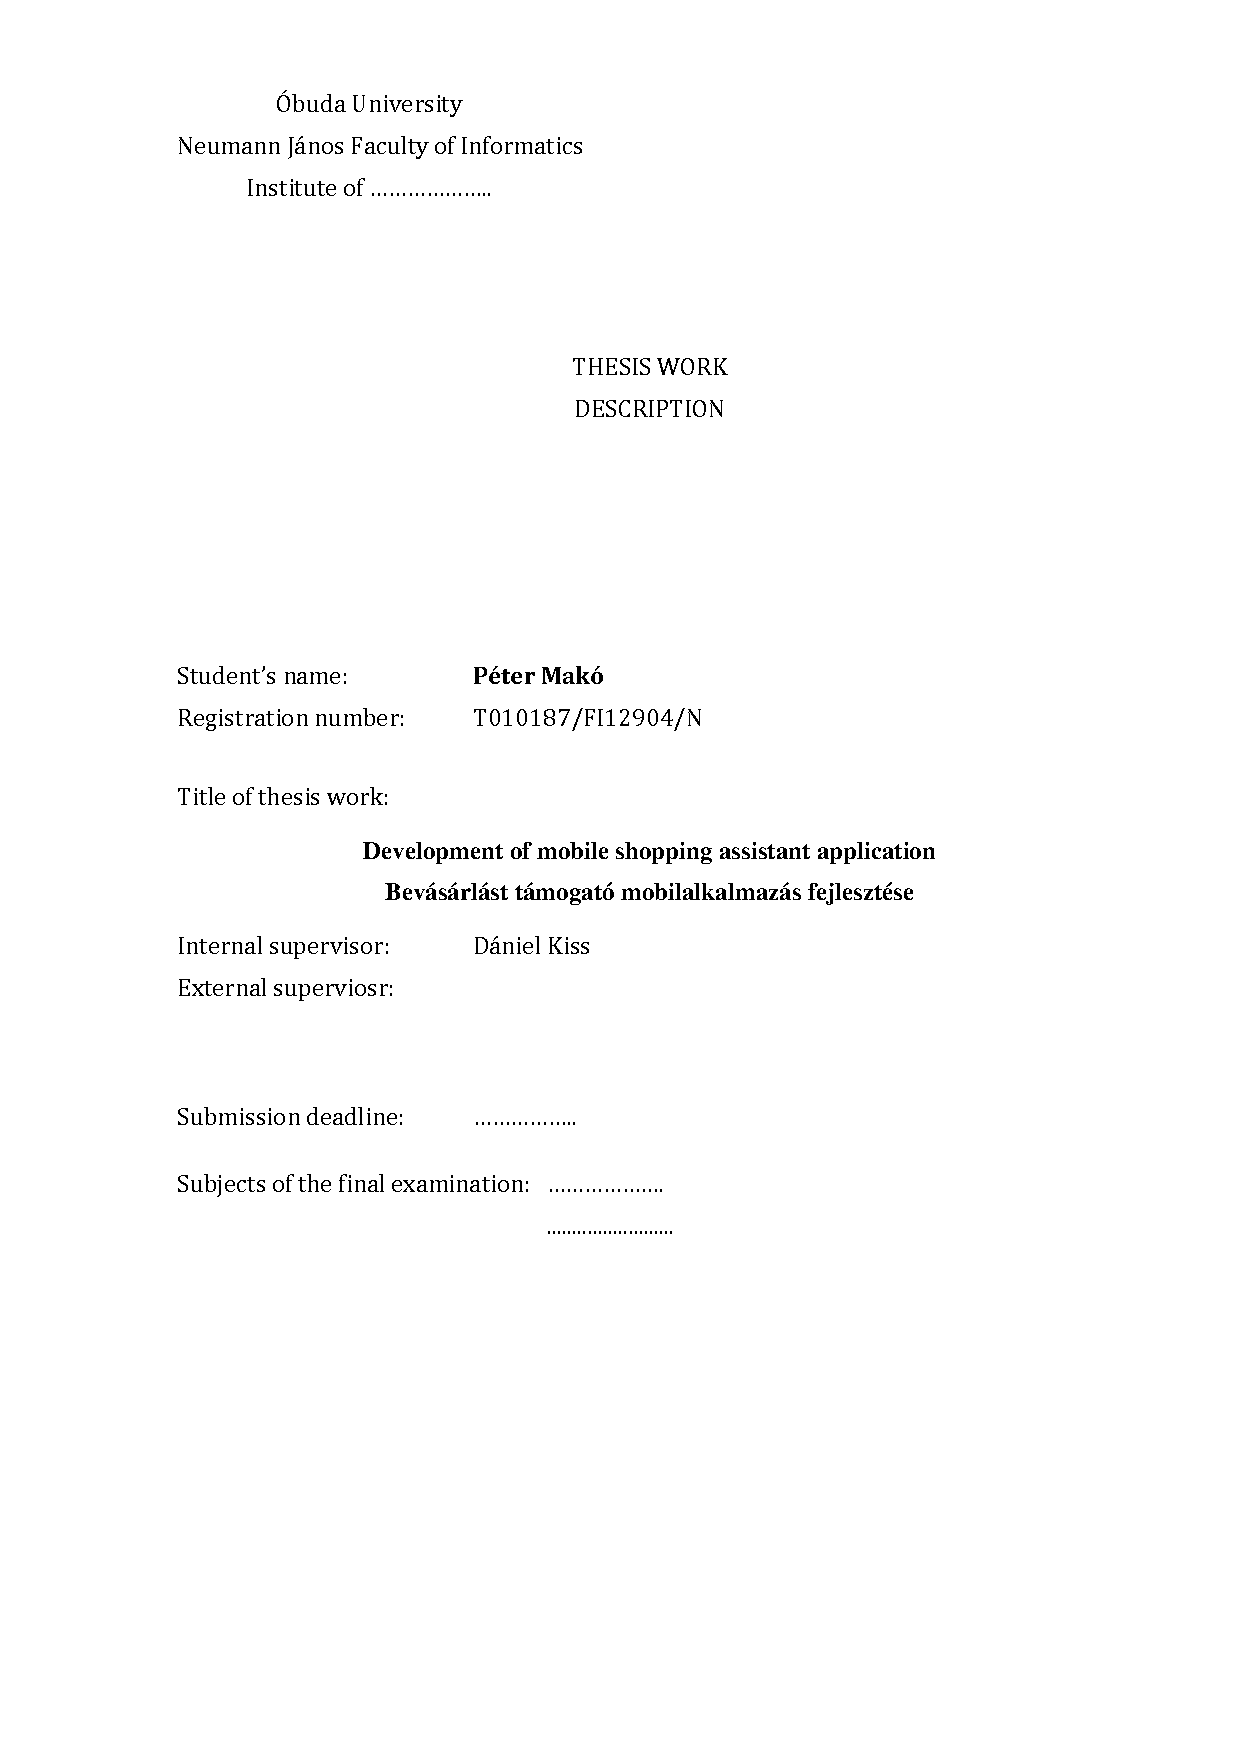
\includepdf[pages=-]{includes/feladatlap.pdf}

\includepdf[pages=-]{includes/nyilatkozat.pdf}
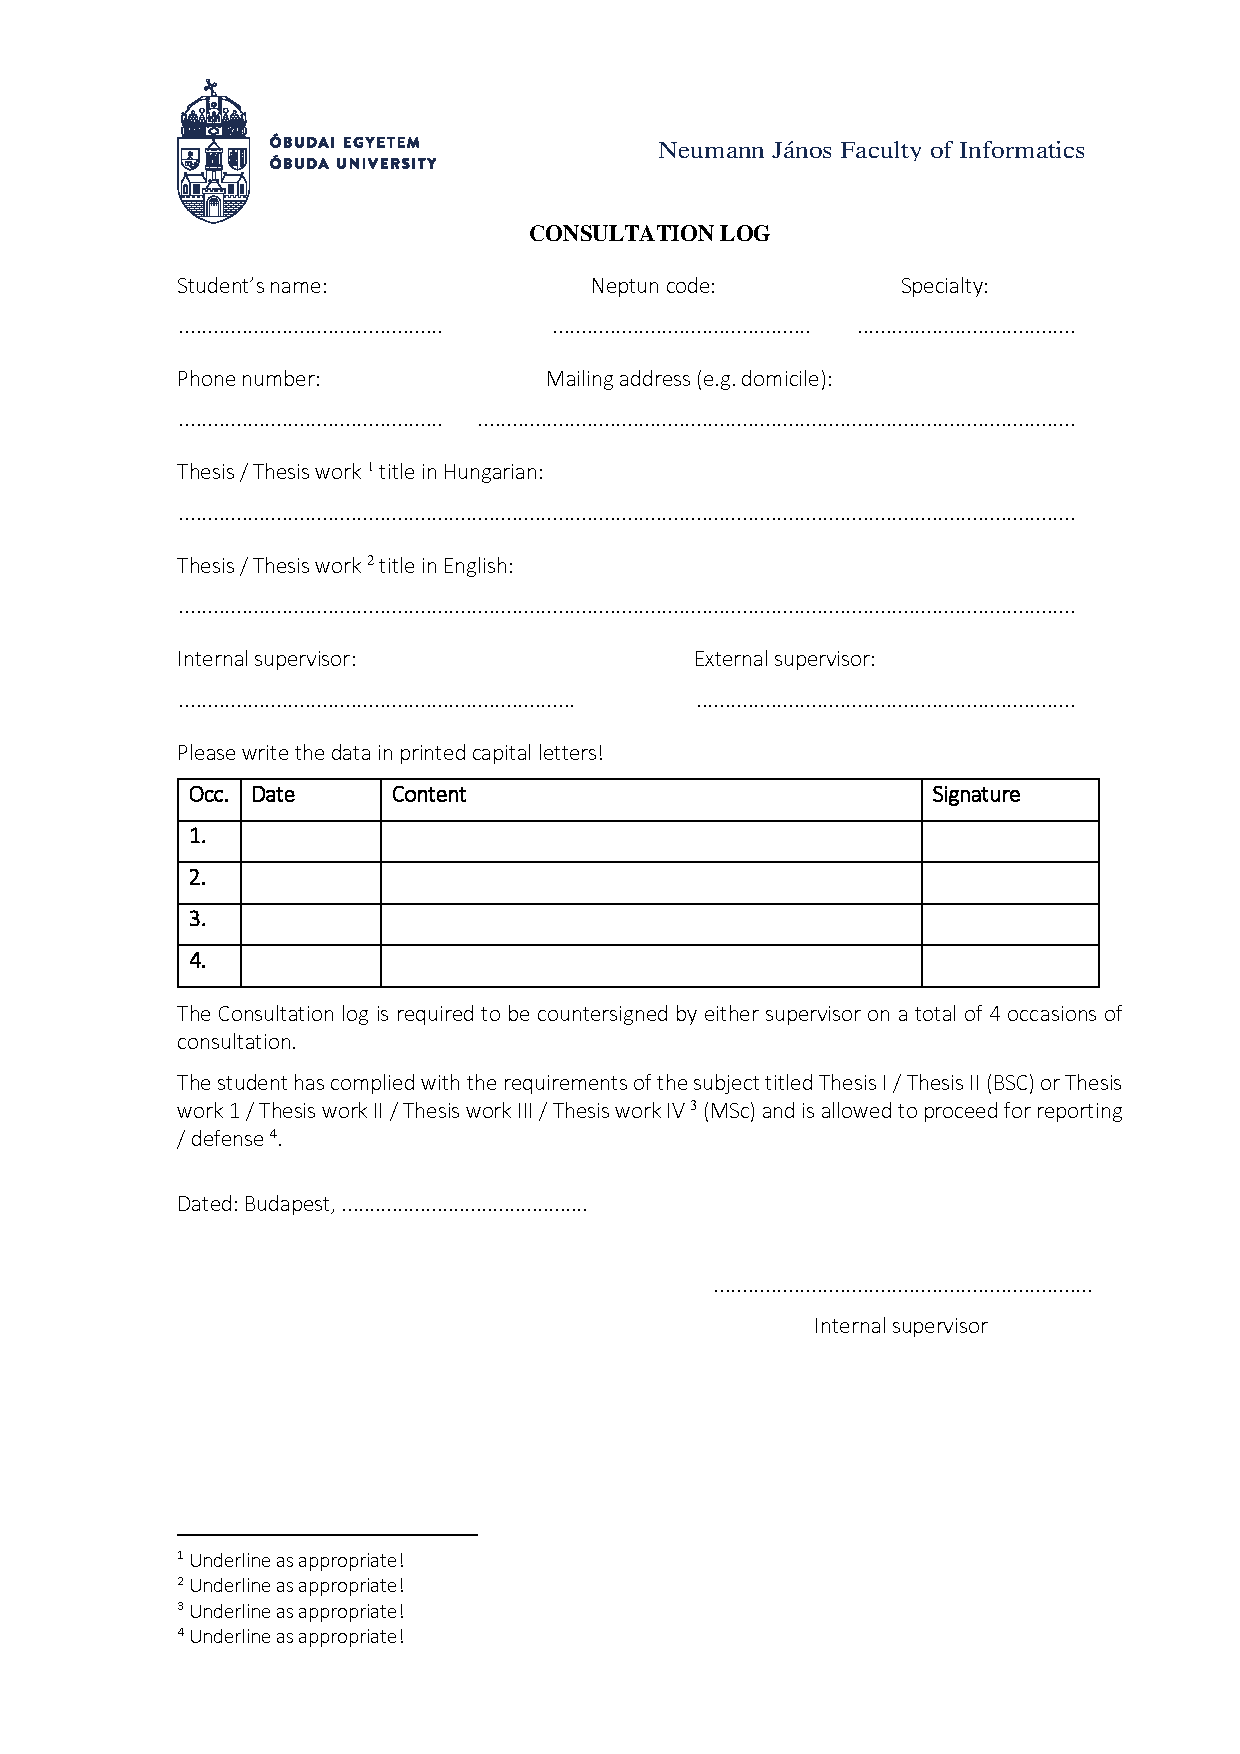
\includepdf[pages=-]{includes/konzultacios_naplo.pdf}
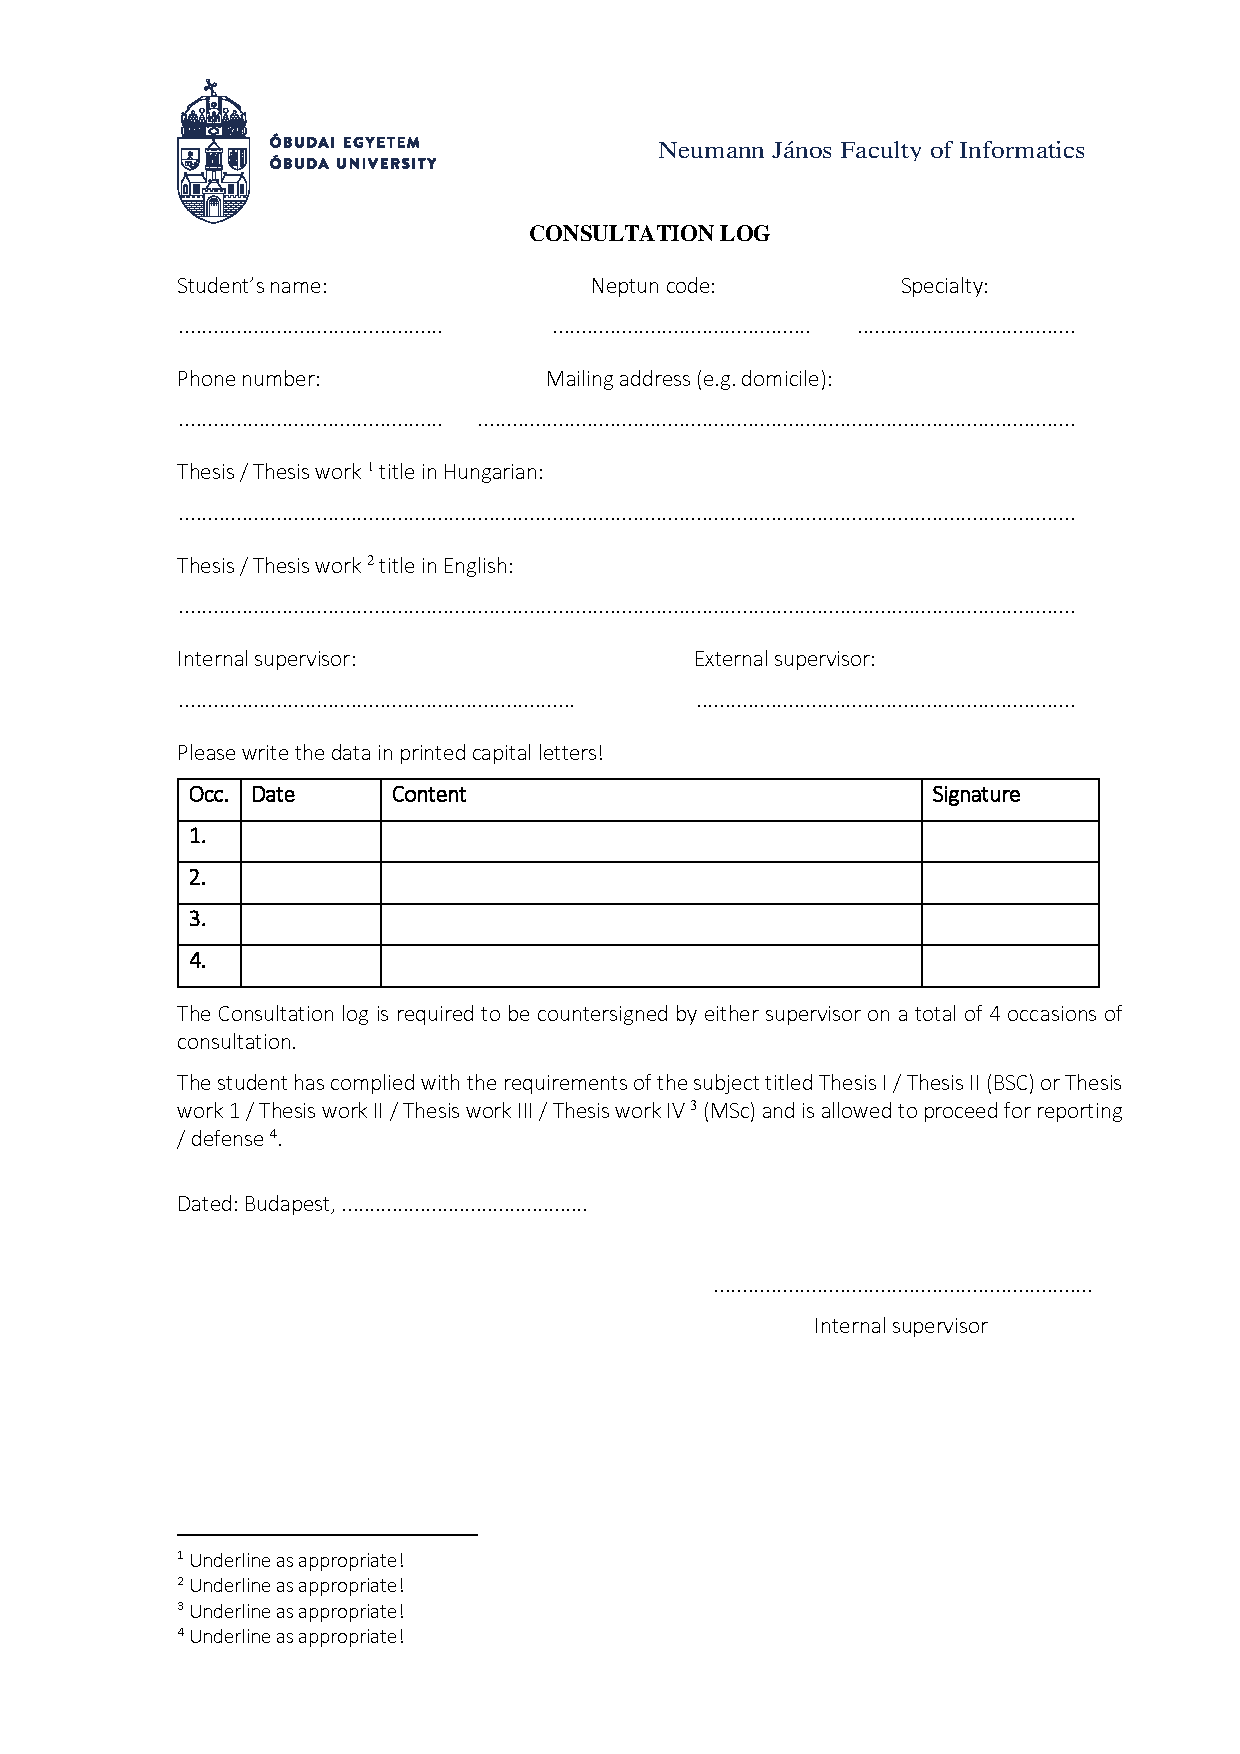
\includepdf[pages=-]{includes/konzultacios_naplo.pdf}
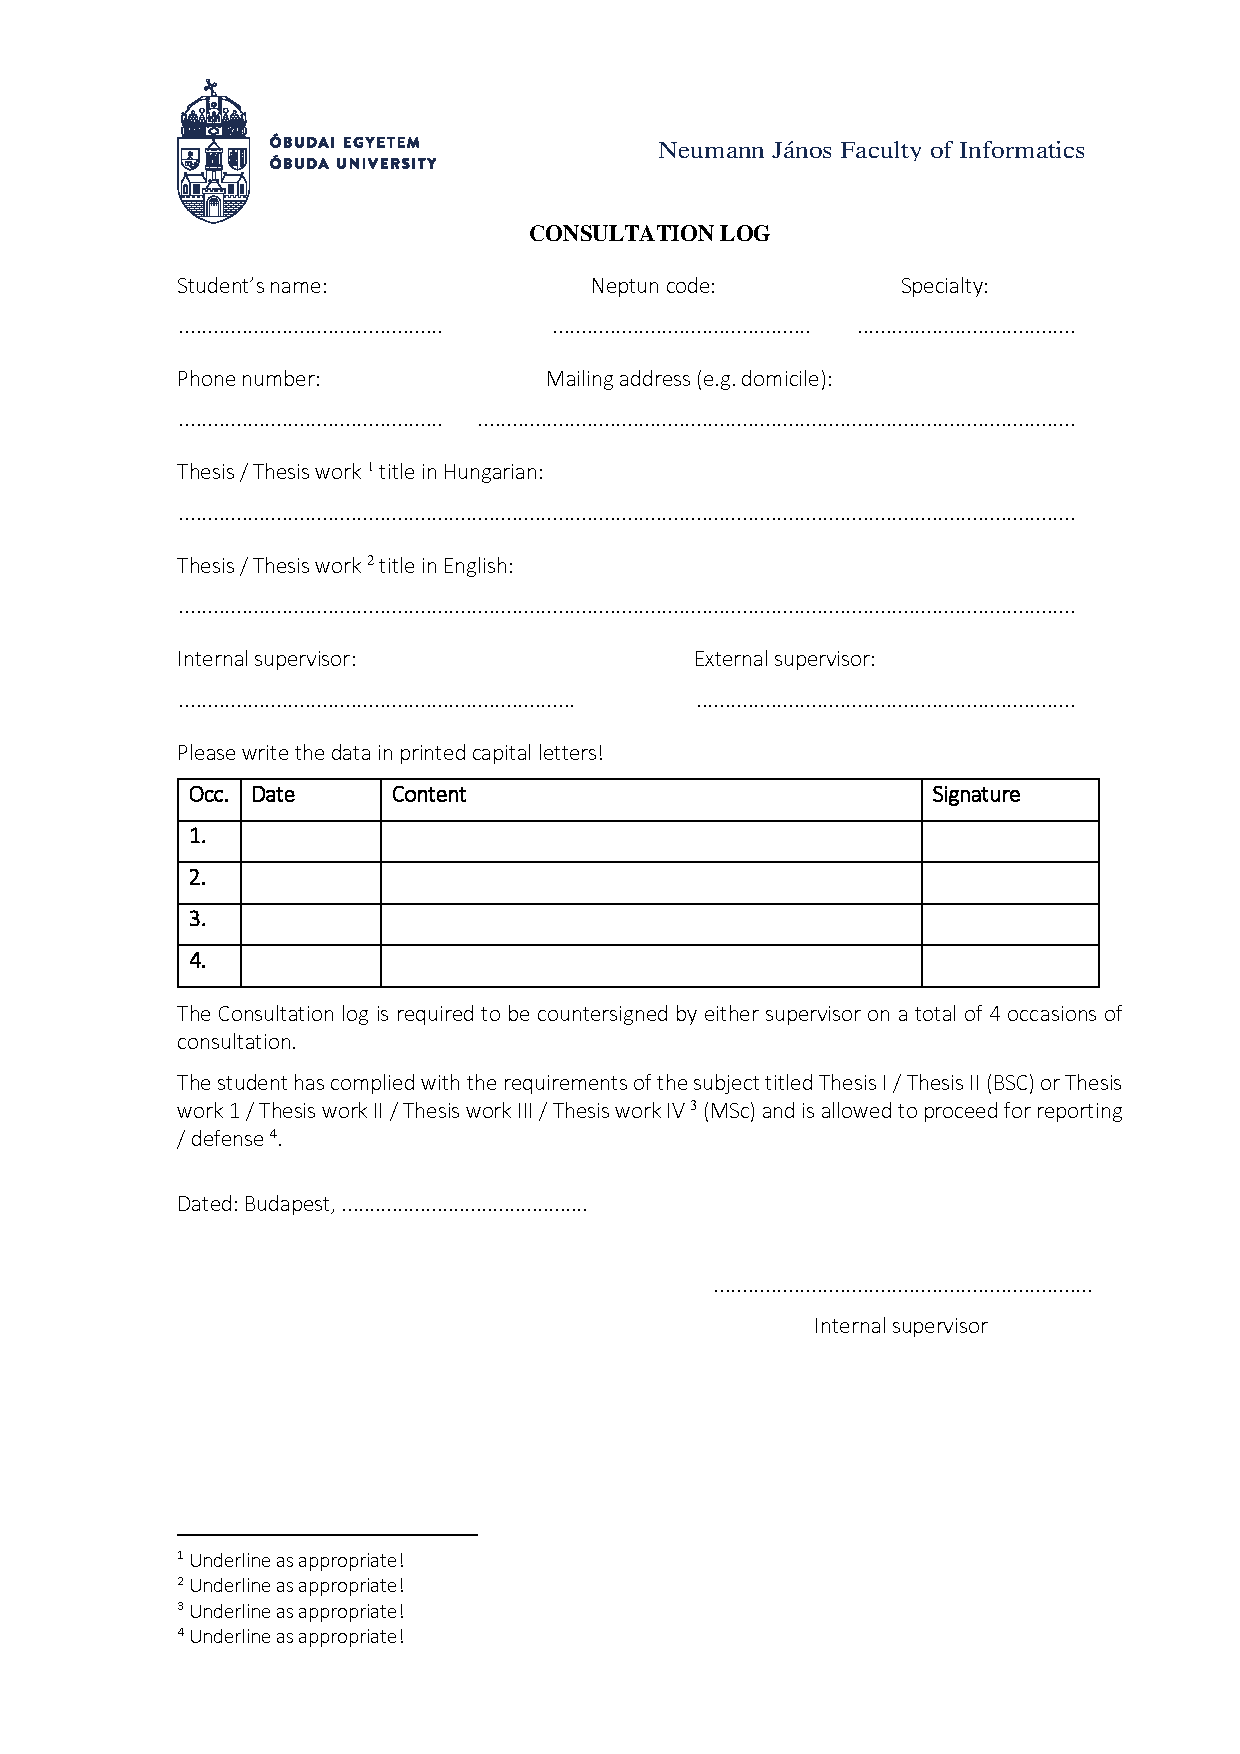
\includepdf[pages=-]{includes/konzultacios_naplo.pdf}
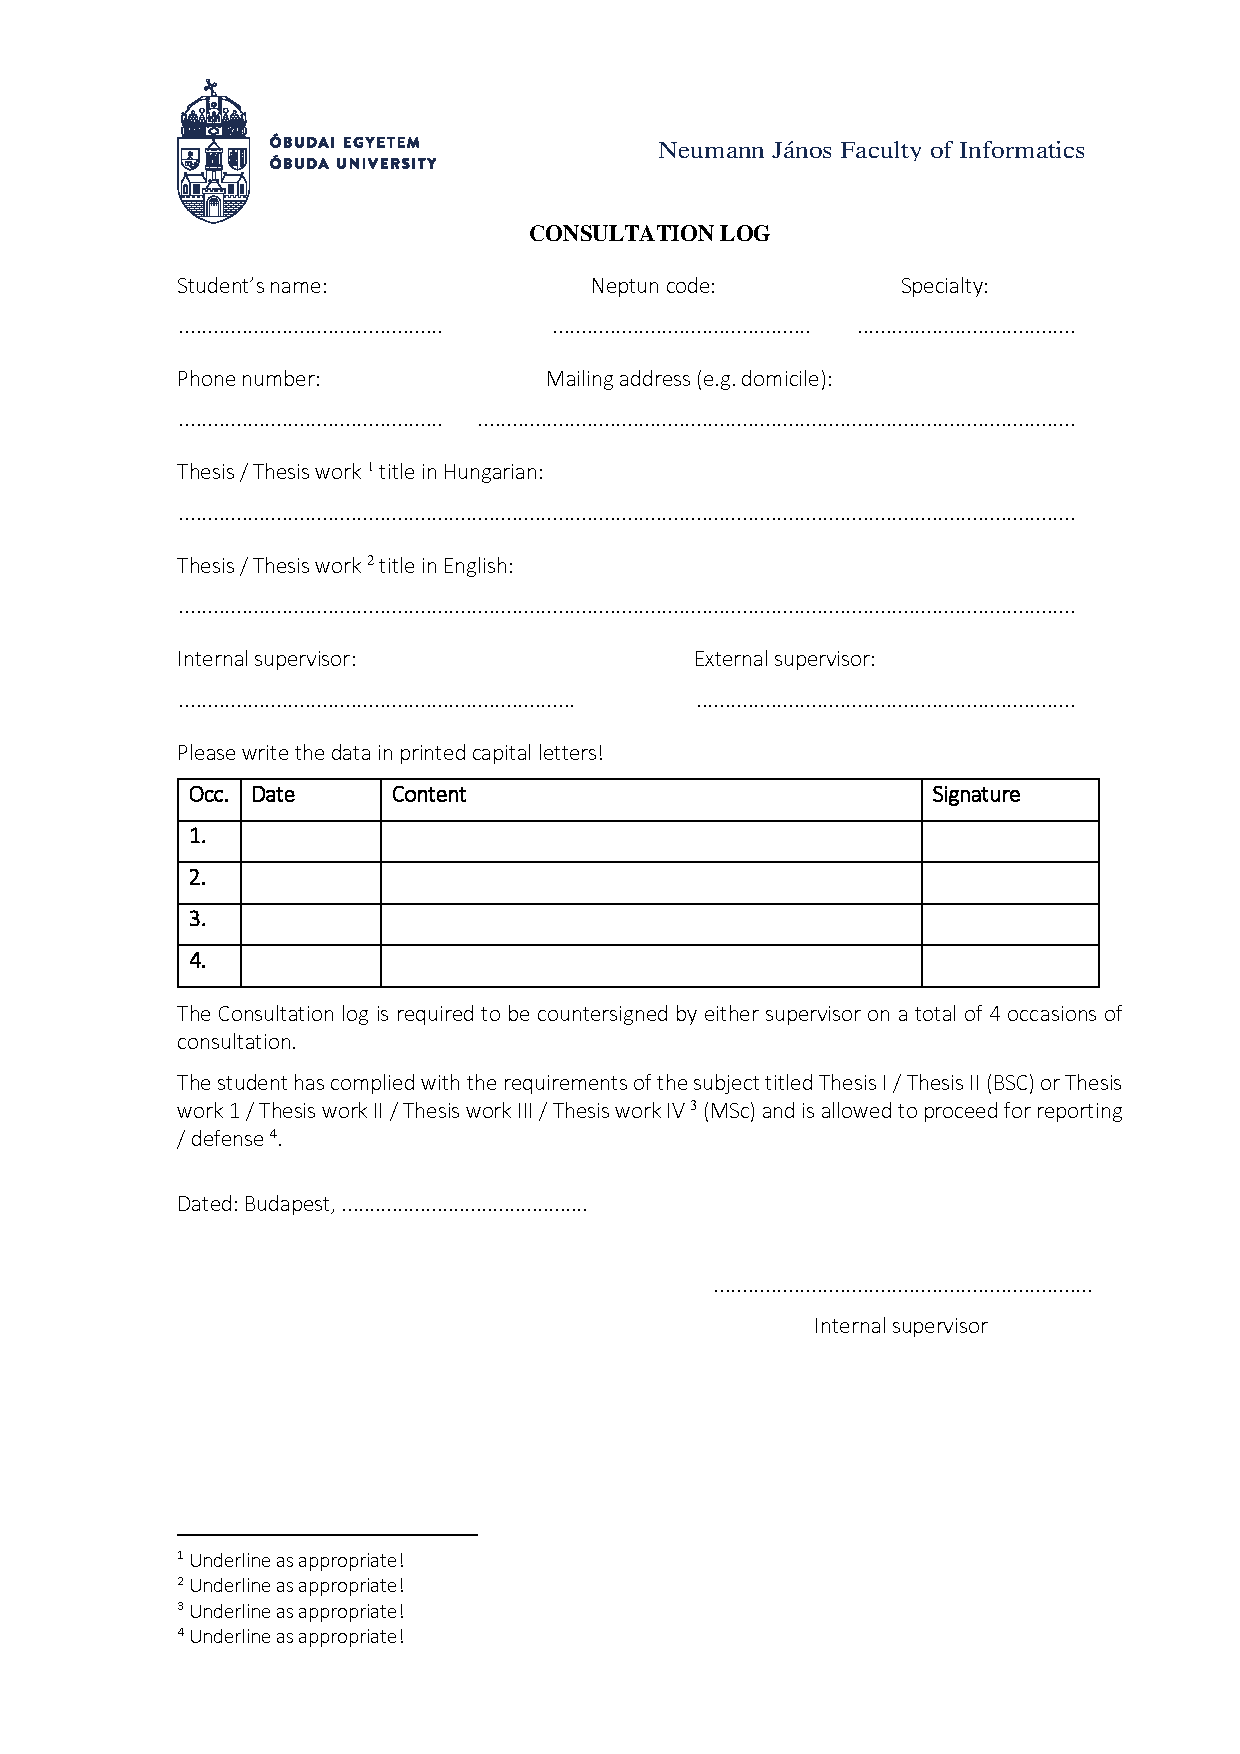
\includepdf[pages=-]{includes/konzultacios_naplo.pdf}
\newpage
\tableofcontents
\newpage

% csak a tartalomjegyzék után kezdődik a számozás
\pagenumbering{arabic}


% -----------------------------------------------------

% ITT KELL HOZZÁADNI A FEJEZETEKET, CÍM NAGYBETŰVEL:

\clearpage
\section{INTRODUCTION}
The purpose of this thesis work is to explore the topic of creating a mobile application that would make people's lives easier when it comes to shopping. With the enormous growth of the competitiveness of the retail market, as well as e-commerce, customers are often left confused whether they would be better off just shopping in the nearest supermarket or rather travel to another one that is further away, but may offer better prices. Implementing a solution for this problem has the potential to become valuable in the eyes of confused customers, who would like to make informed decisions regarding their shopping habits.

Elaborating on the previously mentioned issue, the consumers often face multiple challenges when it comes to a seemingly easy task like shopping. Without information on prices, decision-making is only affected by factors like travel time and personal preference. For this reason, shopping can lead to overpaying for items or not finding the preferred brand or good in the selected store. The process can also become more time-consuming than expected, since there is no guarantee that the customer will only have to visit one shop. Big differences between retail prices can also raise trust issues and misconceptions among customers. Additionally, from the retailers perspective, coming up with the right pricing strategy can be hard, when the factors affecting the customers' decisions are unclear.

The development of such application can potentially result in numerous benefits for both the customer and retail side, such as clear comparisons between different retailers, a more transparent way of pricing the goods, efficient adaptation to the newest valuation trends, customer oriented marketing and the possibility to reduce the time spent with shopping. All of these would result in customers who are aware about the stocks and prices of these retail shops, leading to them making well-informed decisions when choosing shopping habits, as well as getting better prices than ever, because of the fiercer contest on providing the best prices.

The idea of making the life of consumers easier has been around for a while now, but many times they are web-based, meaning that the user experience is not going to be as optimized and straightforward as a dedicated application's case. Furthermore, these applications are usually targeted for international customers, or for those of other nationalities, not to mention that websites usually lack the possibility of searching for bar codes, let alone scanning them for an easy and fast experience.

Implementing the idea for this application requires coming up with all the possible use cases, a well planned  software architecture, a seamless development process, and the thorough testing of the end product. 

Within the scope of this thesis work project, an application will be designed which will provide the user with functions such as using the camera for scanning the bar code of an item, searching for these items with this code or product name, getting prices from various retailers. Moreover, the application will try to give personalized recommendations for the user on where to shop, depending on the goods availability, prices and distance of the shops.

While the primary aim of this project is to target Android devices, for future possibilities it might be more desirable to develop the application using a platform independent approach, like Xamarin. For achieving the desired functionality, there is a need for numerous APIs to provide relevant data on product information, prices as well as the distance between the user and surrounding shops. The testing of the product will be done through multiple approaches to ensure a seamless user experience.

In conclusion, this easy and accessible way of price comparison between shops, brands and goods can lead to an improved consumer culture, where both retailers and customers can make informed decisions. In the following chapters, a detailed examination will be provided on the topic of the importance of transparent price comparison, relevant fields and existing solutions, as well as outlining the concept of the project application, planning and executing the implementation, and finally testing the end product.





\clearpage
\section{BACKGROUND}
The development of barcode technology, as well as the upbringing of handheld software solutions already have noticeable effects on how we shop in our favorite stores. Many retail shops have already implemented self checkout services and handheld or stationary devices, which provide information on the scanned item. Taking this technology one step further will lead us to mobile applications. Out of many already existing programs, finding a Hungary-specific mobile application with such functionality is rather challenging.

\subsection{History of Barcode Technology}
The invention of barcode dates back to the 1940s, when Bernard Silver and Norman Woodland came up with the patent for a system that automatically read product information, using ultraviolet light and ink patterns \cite{barcode2023}. However, only after the introduction of Universal Product Code (UPC) in 1974 did it become widespread in retail industry \cite{weightman2015}. Since then, multiple new types of barcodes emerged, such as the Quick Response (QR) code, which is able to store substantially more information and is faster to read than the original version \cite{densowave2011}. 

\subsection{Evolution of Mobile Devices and Barcode Scanning Applications}

Since the mobile devices come with high-end cameras and very high computational capabilities, they led to the possibility of developing applications, that are capable of scanning the barcodes on products and then providing them with useful information about them, like details, ratings and prices \cite{chen2012}. The first famous pioneers were RedLaser and ShopSavvy, whose popularity has been mainly connected to the users ability to save time and money using them for comparing product details and prices \cite{rao2011}.

\subsection{Relevance of Price Comparison in The Retail Industry}

A highly competitive market results in price comparison becoming an essential aspect of modern shopping experience, since an increasing majority of consumers strive to become more informed about the products and their details before making a decision on where and what to shop for \cite{huang2006}. This trend is fueled by e-commerce, widespread mobile internet access and an increasingly high competitiveness in retail market \cite{pentina2014}. Using these applications led to retailers being forced to use different pricing strategies, as well as investing in digital technology to provide the customers with the required transparency and comfort \cite{grewal2011}.

\clearpage
\section{ANALYSIS OF PURPOSE-RELATED SOFTWARE}\label{related}
The technology of scanning barcodes has evolved since inventing it. Nowadays, these codes have multiple types, such as the one-dimensional, linear barcodes, the two dimensional barcodes, like QR code and Data Matrix \cite{}. These codes are scannable with either a special scanning device, a mobile phone or some other imaging devices, which have a software capable of deciphering these codes installed.

While websites with capabilities to track product details do it so using a code from user input, the advent of smart phones with built-in cameras has led to designing applications which are capable of fast scanning of barcodes and then fetching details about the given item \cite{}. Throughout the years many libraries and APIs have been developed to make integrating such functions into mobile applications easier.

No matter whether the web or the mobile approach is used, these applications could provide crucial functionalities when it comes to the rising trend of barcode scanning and real time price comparison. Soon after realizing this, many companies decided to provide users with solutions with such functionalities. However, to come up with something innovative, we have to understand the background and functionality of already existing software. This chapter will give a comprehensive analysis on multiple similar or functionally related solutions, such as PriceGrabber.com, Google Shopping, RedLaser, PriceRunner, ShopSavvy, and Hungarian ones like Arukereso.hu and Cashmap.hu. Considering these implementations, my goal is to develop an application that will stand out in the competitive market.

\subsection{PriceGrabber.com}

Established in 1999, PriceGrabber is one of the oldest price comparison services out there. Naturally, back then it started off as a website, but later a mobile application was developed as well. The service lets customers get free price information on millions of products, while getting its profit from countless merchants paying for each lead. In 2005 it was acquired for 485 million USD by Experian and was expected to grow substantially in the next five years \cite{Forbes2005}, then later another acquisition was made by Connexity in 2015 and it has been owned by them ever since \cite{Connexity2015}.

The success of PriceGrabber originates from its ability to adapt through the evolution of the technology industry. Eventually a smart phone application was released, first for iPhones, later for android devices, which enabled the user to access the same functions as from the website. It was designed to host an increasing number of users and allowed them to read product reviews, create a favorite list and compare prices. Laura Conrad, the president of PriceGrabber, stated that this application was developed to remove the boundaries between online and offline shopping, targeting the growing number of people of mobile shoppers \cite{HarnickPriceGrabberApp}.

\subsection{Google Shopping}

Possibly the best known e-commerce platform, Google Shopping took off in 2002. It has been a major part of the search engine and google ads ever since. Whenever a user searches for something retail related, google gives them the best matches and options alongside with sponsored ads.

On the business side, the target audience is made up mainly from advertisers and sellers, providing them with different methods to promote their goods and services. The service is based on a Cost-Per-Click model, which means that Google gets paid for every click that users make on a company's ad. Ranking is affected by multiple factors, such as relevance to search keywords, how well does it fit into the user search history and last, but not least on how much does a company pay for their product to be ranked higher, in which case google differentiates it with a "Sponsored" flag from the other ads.

From the consumer's point of view, the service provides personalized ads based on factors like demography, search history and interactions with Google services. This kind of personalization ensures relevance and user engagement leading to a competitive, yet rewarding environment.

On the technical note, the service is backed up by Google's robust systems. It is strict with forcing the retailers adhere to Google's policies before letting them post their ads. It uses machine learning models to maximize the relevance for users. Google Shopping also gives a lot of personalization possibilities for the consumers, such as filtering the products, depending on the category, brand and more importantly price. The service also incorporates reviews from multiple sources to assist a better understanding on the benefits and drawbacks of choosing certain products. The process ends with clicking an ad, where Google's business model steps into action and the seller pays them for the successful redirection to their product's page. \cite{Google2023}

\subsection{RedLaser}
Although it has been discontinued since and taken down from both App Store and Google Play Store, RedLaser, acquired by eBay in 2010 was one of the most popular barcode scanner and price comparison application using various services of its acquirer.

In 2011 RedLaser 3.0 rolled out, with integration of various eBay mobile services, creating a great user experience for shopping based on price comparison. The application utilized Milo's local inventory data to enable price comparison among online and offline stores and PayPal's mobile express checkout for a secure payments.

Although the earlier versions were well known too, the application's popularity rapidly grew thanks to the new, unique features introduced by this update. These included the ones mentioned in the previous paragraph, along with a refined user interface, which made scanning and creating lists and QR codes much easier. It also enabled users to share categorized shopping carts through Facebook, SMS and e-mail.

In RedLaser's prime it was downloaded tens of millions of times, however, after many years, it could not keep up with the competition and was discontinued.

\subsection{PriceRunner}

PriceRunner, founded in 1999, is an independent price comparison service offering a platform to help consumers make informed decisions about their purchases in the United Kingdom. Using the service is free of charge and it provides daily updates on millions of products regarding their price and details. Even though the in 2022 PriceRunner was merged into Klarna, PriceRunner managed to keep its core values, which are independence, credibility and unbiasedness, therefore highly contributing to smarter e-commerce decisions. \cite{PriceRunner2023}

Much like Google Shopping, PriceRunner uses the model of affiliate marketing \cite{PriceRunnerTerms2023}. This is commonly known as the Cost-Per-Click model mentioned earlier in Google's case. The service gets paid by affiliated customers after each successful referral. It boasts a unique feature, buyer protection, beneficial for the users in case where the retailer does not meet their statutory obligations. Buyer protection is a free service for all users, providing financial coverage up to five thousand pounds, in case of a purchase from any of PriceRunner's associated retailers. \cite{PriceRunnerFaq2023}

PriceRunner offers their services both on their website and on their mobile application. Being UK's largest product and price comparison service, it lines up more than 2.6 million products. The app provides the users with smart features enhancing their shopping experience. These functions include but are not limited to using its built-in barcode scanner to find certain items, compare their prices and upcoming deals on the product. It also equips the customer with price alert settings, so that they will be notified about the drops in price. The great user experience is maintained by continuously updating pricing data from thousands of retailers ensuring that the price comparisons are up-to-date. Additionally, users can create lists of certain products they like and monitor their prices and deals on them. \cite{PriceRunnerApp2023}

\subsection{ShopSavvy}

Possibly the best application out there in this topic would be ShopSavvy, developed by Monolith Technologies Inc., which has been around since 2008. It was one of the first applications developed for both iOS and Android. It is available for all popular browsers, such as Microsoft Edge, Google Chrome and Safari as an extension plus as a mobile application for iPhones, iPads and all sorts of Android devices. The service's goal is to provide the user with the best possible prices on all kinds of items, with promoting fairness, being customer oriented and independent. \cite{ShopSavvyAbout}

ShopSavvy evolved from a barcode scanner app to a service that rounds up tens of thousands of retailer partners and covers all aspects of price comparison such as sales, markdowns and coupons to provide the best possible price for the user. It monetizes the platform in two major ways. Firstly, they target users with personalized offers through the service and if this offer catches the eye of the consumer enough for them to make a purchase, the company will earn commission from that sale. Secondly, it generates revenue from advertisers using the platform to reach even more costumers, therefore serving as a mediator platform between retailers and customers. ShopSavvy considers itself as a product search company, with an aim to match the consumers with their desired products for the best possible price. CEO John Boyd explains that the best strategy for competing with giants like Google, Facebook and Amazon is to constantly innovate and come up with unique value propositions. \cite{PymntsShopSavvy}

The company rounds up multiple software solutions for using their service. Meanwhile the browser add-ons are for online shopping, usually for non-essential items, the application shines when it comes to grocery shopping with barcode scanning possibilities. The service itself gathers information from over 30 thousand retailers, both online and physical stores through two methods. Firstly, it partners up with retailers, so they would provide information about prices and sales, secondly it uses web crawling and scraping to find information on products from non-partner stores. The data about items and prices are collected real time, meaning that the user is provided with the most up-to-date information. The search and scraping work using both barcodes and keywords to find accurate results. The hardships of the recent lockdowns forced ShopSavvy to adapt and come up with an in-stock inventory tracking, which lets customers locate hard-to-find items in stock. It offers an easy to navigate platform for users to discover, shop and save. It aggregates product information from a wide-variety of network sources to provide the customer with unbiased data on deals, ratings and reviews. The platform also provides a place for the users to form a mobile shopping community that extends beyond the general concept of such applications. \cite{shopsavvy2020}

\subsection{Arukereso.hu}

Arukereso.hu is a market-leading price comparison website in Hungary with operating in two additional countries, namely Romania and Bulgaria. It started off as a small service maintained by two individuals in 2004, listing and comparing a few items from a few webshops around the dawn of internet shopping. In 2009 it was acquired by Allegro Group, but the current state was established in 2016 when another acquisition was made by Rockaway group. \cite{arukeresoLinkedin}

Arukereso.hu is similar to previous price comparison websites. It uses the same Cost-Per-Click affiliate business model to get revenue from partner retailers or sometimes extra for actual purchases through them. What makes them unique on the market is the fact that it is the best-known website with such functionality in Hungary, where many other companies do not operate yet, coupled with providing an all-around unbiased review system, where users can rate both the product and the seller. This system solves the asymmetry when it comes to cheap prices and questionable sellers and also ensures a more trustworthy line-up of stores. \cite{karacsony2019}

The previously mentioned review system comes into play after a user makes a purchase. They get asked to provide feedback on the product they purchased along with the seller they bought it from. The ratings are designed to allow replies, that way the stores or other users can clarify reviews in certain cases. The site also provides an option to ask questions about certain products, which paired with the review system provides a platform for a community of mindful customers. An additional layer of trust is provided by a "Trustworthy Shop" badge, which is only achievable with a high number of positive reviews left by actual users \cite{arukereso}. 

\subsection{Cashmap.hu}

With unfortunately less public information available comes another Hungary specific shopping assistant, Cashmap.hu. It is a newly launched startup designed to transform the way Hungarians shop. It encourages their users two make well informed and rational decisions about where they shop and what they buy. It provides information on prices and discounts for up-to 9 popular supermarket chains. The service is completely independent, it is not by any means in business relationship with the stores they provide information about. \cite{maradokapenzemnel2021}

Their service is a web-based application with features like searching for the desired product and compare prices among multiple stores. The user can also put a personalized shopping cart together and calculate which store offers the best final sum. If the shopping cart contains items the user does not need right away, there is a possibility to move them into a "Later Cart" to wait for future discounts. The service uses web crawling and scraping, using multiple sources, including in-store surveys, online sale fliers, online store interfaces and internet searches to ensure that the information provided is accurate and up-to-date. \cite{maradokapenzemnel2021}

\subsection{Conclusion}

After a thorough examination of already existing software solutions for this specific problem, it is clear, that the market is somewhat saturated and that there are multiple notably great features implemented in the analyzed applications. However, it is important to mention, that while some have great functions, there are those that do not exist anymore and others, which do not necessarily target the same demographics. 

Since the idea for creating this application came from the current situation in Hungary, specifically with grocery shopping in mind, while the international and other region specific implementations are important from a technical point of view, they do not affect the market and target audience in question yet. On the other hand, both of the Hungarian websites mentioned provide features that are on par with some of the ones I am planning to implement. This also encourages a solution for this problem that places the application in a unique spot on the market. A key difference will be accessibility, since the software will be a dedicated smart phone application instead of a generic website solution. 

Finally, the following conclusion can be drawn from this analysis. For the upcoming application to be successful among the target audience and in the target market segment, it needs to combine the best of all worlds, meaning that it should line-up a number of features not yet available in our region, build on the existing and well-established model, pay close attention to the reactions and requests of the user-base and adapt if needed. In the upcoming chapter I will carefully develop the vision for this application and its aspects.

\clearpage
\section{VISION}
\subsection{Introduction}

\subsubsection{Purpose}
This chapter serves as an outline for the vision for "BargainScan", an innovative mobile application to help customers save on everyday shopping tasks and to spend on what really matters. This vision will guide the reader through all key aspects of the development of the upcoming application such as opportunities, challenges, target audience, benefits and features of the software. It will act as a reference for all stakeholders involved in the project.

\subsubsection{Scope}
"BargainScan" is an upcoming mobile application aimed to make grocery shopping a conscious and informed act for Hungarians by providing a platform for scanning and searching for products, comparing the prices across supermarket chains and retail shops, providing calculations on shopping lists in different stores, listing shops sorted by travel distance and affordability and building an aware shopping community in Hungary.

\subsection{Positioning}

\subsubsection{Business Opportunity}
The global and local e-commerce and retail market has shown significant growth in the past decade. With the increasing adoption of smart phones into people's everyday life, especially concerning their shopping habits, it is clear that there is an opportunity for developing applications to assist them with these daily tasks. "BargainScan" is aimed to fulfill this mission by offering a comprehensive and versatile solution, equipped with a user-friendly and straightforward interface.

\subsubsection{Problem Statement} 
As stated in the previous chapter (\ref{related}), while the global market has many solutions for shopping assistants, many lack important features or are implemented as websites which are less accessible than a mobile application. Additionally, even if there are adequate solutions on the global market, they simply are not meant to be used in Hungary, since they only list products and retailers that are commonly not available in Hungary with many times not even supporting this region.

Currently there are no mobile applications with such purpose on the Hungarian market. On the other hand, there is a series of established that more or less offer useful features for the users, which share the problem of not being accessible enough, especially for older folks, who need a very straightforward way of accessing the software. Moreover, neither of the existing applications seem to offer a solution that covers the whole process of finding the best products and prices and planning the next shopping spree carefully including various factors, for example travel distance or how crowded the place is.

\textbf{Customer Perspective:}
They need a comprehensive and intuitive application that helps them find not only the best prices, but also the best way of shopping by filtering out stores that do not fit into their desired characteristics. Additionally, they need a platform where they can build a community to rate and share insights on certain products and sellers.

\textbf{Seller Perspective:}
Businesses need a platform to provide their up-to-date information on, therefore reaching potential customers, increasing the likeliness of being chosen by the users and making their prices competitive against other companies.

\subsubsection{Product Position Statement}

"BargainScan" will be an application designed for money-conscious individuals who seek a comprehensive, clean and user-friendly solution for the stated problem. Unlike existing applications, its primary aim is to cover not only a few, but most aspects of the shopping process, from searching for products through their name or barcode, finding the best prices, filtering shops and products on certain terms, getting personalized recommendations and reading unbiased ratings and opinions on products and businesses. 

While realizing all of the features which will make this software a unique solution, it is important to provide an application with a straightforward and easy-to-use interface for the target audience, because accessibility plays a key aspect in the adaption process, hence in the general success.

\pagebreak

\subsection{Market Analysis}

\subsubsection{Market Demographics}

The growth in the competitiveness of retail and e-commerce led to a situation where customers are overwhelmed by choices, but they are unable to make informed ones due to lack of information about stores and products. The application is aimed to target the individuals with the desire to make conscious decision about their shopping habits. In the table (\ref{tab:md}) below, I will list the key aspects of the target market demographic.

\begin{table}[h]
	\centering
	\begin{tabularx}{\textwidth}{|p{3cm}|X|}
		\hline
		\textbf{Aspect} & \textbf{Description} \\
		\hline
		Age Group & The target age group is between 12 and 99, comprising Generation Z, millennials, Generation X and even baby boomers, meaning that the application is for everyone that seeks help with making informed decisions. Additionally, the intuitive design of the application makes it suitable and accessible for all age groups. \\
		\hline
		Income Level & The application can prove to be useful for customers across various income levels, offering features for comparing prices and finding the best deals, which is particularly appealing to middle-income earners. \\
		\hline
		Geographic Location & The shopping assistant app is primarily targeted towards all areas of Hungary with internet connection and grocery stores available. \\
		\hline
		Shopping Habits & The primary user base is expected to be mostly made up from millenials and Gen X members, since they are shopping for groceries on a daily basis, are the most comfortable using technological solutions in their everyday routines and value convenience and time saved. \\
		\hline
		Technological Proficiency & The application will be developed for smartphone users with different levels of technological proficiency. The user-friendly interface is set out to ensure that every individual will be able to wrap their head around the concepts of the application.\\
		\hline
	\end{tabularx}
	\caption{Market Demographics}
	\label{tab:md}
\end{table}

\pagebreak

\subsubsection{Porter's Five Forces Analysis}

To better understand the competitive dynamics and attractiveness of the proposed "BargainScan" application on the market, Porter's Five Forces analysis will be utilized in the table(\ref{tab:pffa}) below, encompassing the threat of new entrants, bargaining power of suppliers, bargaining power of buyers, threat of substitute products or services and rivalry among existing competitors.

\begin{table}[h]
	\centering
	\begin{tabularx}{\textwidth}{|p{4cm}|X|}
		\hline
		\textbf{Force} & \textbf{Impact} \\
		\hline
		Threat of New Entrants & The threat of new entrants is high due to low entry barriers in the app development industry. In case of a successful counterpart for the application could mean serious competition.\\
		\hline
		Bargaining Power of Suppliers & In the context of a barcode scanner, price comparison and shopping assistant application, suppliers could be businesses whose products are listed. They have low bargaining power as there are numerous online and offline retailers and not being present could lead to missing out on potential customers. \\
		\hline
		Bargaining Power of Buyers & Buyers have moderate bargaining power. As of now, there are only websites available in Hungary for this specific purpose, with more or less relevant features. \\
		\hline
		Threat of Substitute Products or Services & The threat is moderate as there are other ways consumers can seek shopping assistance, such as through the mentioned websites, direct e-commerce platforms, but currently there are no Hungary specific applications on the market. \\
		\hline
		Rivalry Among Existing Competitors & The competition is fierce in the digital marketplace industry, the application needs to provide unique value proposal to be potentially considered instead of other existing solutions. \\
		\hline
	\end{tabularx}
	\caption{Porter's Five Forces Analysis}
	\label{tab:pffa}
\end{table}

\pagebreak

\subsubsection{PEST Analysis}

The external macro-environment in which "BargainScan" is set out to operate in can be explored by using the PEST analysis, cosidering political, economic, sociocultural and technological factors. The evaluation of these factors are visible in the table (\ref{tab:pest}) below.

\begin{table}[h]
	\centering
	\begin{tabularx}{\textwidth}{|p{2.3cm}|X|}
		\hline
		\textbf{Factor} & \textbf{Impact} \\
		\hline
		Political & In Hungary various legal regulations affect data privacy, e-commerce, and internet advertising. Any changes in these policies may impact the operation and strategies of the application. \\
		\hline
		Economic & Economic factors such as income, unemployment rates, consumer confidence influence the way and frequency people utilize this application, the willingness of businesses to advertise their products through this platform will determine the success of the application. \\
		\hline
		Sociocultural & The growth of digitalization in every field of everyday life definitely helps the success of the application, since there is a wider spectrum of people who are ready to use their smart devices to make their lives easier. Additionally more and more people aspire to be more conscious about their shopping habits.\\
		\hline
		Technological & Rapid advancements in technology, such as artificial intelligence, machine learning, and the increasing size of mobile network coverage, can lead to more innovative and valuable features in the application. Cybersecurity on the other hand poses a significant challenge for designing such applications. \\
		\hline
	\end{tabularx}
	\caption{PEST Analysis}
	\label{tab:pest}
\end{table}

\subsubsection{Ansoff Matrix Analysis}

A great tool for further clarification of the potential success of the application is the Ansoff matrix. The table (\ref{tab:ansoff}) on the next page will study the strategies such as market penetration, market development, product development and diversification.

\begin{table}[h]
	\centering
	\begin{tabularx}{\textwidth}{|p{3.7cm}|X|}
		\hline
		\textbf{Strategy} & \textbf{Description} \\
		\hline
		Market Penetration & The application will focus primarily on the demographic of daily grocery shoppers, so it will seek to deepen its influence in this existing market. In order to achieve this, the solution will offer unique features, ensure the best deals and unbiased product reviews. \\
		\hline
		Market Development & The app will be designed to be appealing to not only daily shoppers but also those who seek to spend their money consciously, by making informed decisions. Moreover, upon a successful adaptation in Hungary, an expansion to other geographic regions is considered part of the long-term plan. \\
		\hline
		Product Development & The fast paced advancement of technology draws a path for continuous technological developments, such as implementing artificial intelligence, machine learning, etc.\\
		\hline
		Diversification & Looking towards the future, the application's idea holds possibilities for expanding into other, new markets. Possibly the biggest potential of these opportunities is held by evolving into an application, that much like Wolt or Foodora, would offer delivering the products from an own warehouse or from existing stores. \\
		\hline
	\end{tabularx}
	\caption{Ansoff Matrix Analysis}
	\label{tab:ansoff}
\end{table}


\pagebreak

\subsection{Stakeholder and User Descriptions}

\subsubsection{Stakeholder Summary}

The table (\ref{tab:ss}) below provides a summary for outlining the key stakeholders involved, highlighting their representation and roles in this mobile application project.

\begin{table}[H]
	\centering
	\begin{tabularx}{\textwidth}{|p{2cm}|X|X|}
		\hline
		\textbf{Name} & \textbf{Represents} & \textbf{Role}\\
		\hline
	Users & Individuals seeking a comprehensive shopping assistant & Provide feedback, requirements, test application \\ \hline
		Retailers & Businesses offering product information for customers & Provide feedback, requirements, test application, contribute to product and store data collection \\ \hline
		Developer & Sole technical expert & Design, develop, test, maintain software solution \\ \hline
	\end{tabularx}
	\caption{Stakeholder Summary}
	\label{tab:ss}
\end{table}

\subsubsection{User Summary}\label{ussect}

The table (\ref{tab:us}) below provides a summary for defining the potential users involved, detailing the way they might interact with the application and their representative stakeholders.

\begin{table}[H]
	\centering
	\begin{tabularx}{\textwidth}{|p{2cm}|X|X|}
		\hline
		\textbf{Name} & \textbf{Description} & \textbf{Stakeholder}\\
		\hline
		General Users & Use the application to scan barcodes, search for products, create shopping lists, provide reviews on items and stores, filter stores based on personal criteria & Users \\ \hline
		Researchers & Use the features of the software for market research purposes & Users \\ \hline
		Admins & Manage the application data regarding stores, products and users & Users \\ \hline
		Retailers & Provide data on their business and goods & Retailers \\ \hline
	\end{tabularx}
	\caption{User Summary}
	\label{tab:us}
\end{table}

\subsubsection{User Environment}

Users are primarily individuals seeking an assistant that helps them make informed decisions about the products they buy and about the businesses they shop at. As mentioned in the user summary (\ref{ussect}), the other types of users are researchers doing market research and retailers, who provide information on their business and products. The goal is to provide a user-friendly mobile application, that implements versatile functionality to fulfill all the important use-cases. The general users are expected to use the application both on the go and at home, while other users will probably use it from an office background.

\pagebreak

\subsection{Product Overview} \label{po}

\subsubsection{Product Perspective}

"BargainScan" is a comprehensive shopping assistant application, developed to help making informed decisions for customers across various demographics. Its positioned within the e-commerce market, targeting users with smartphone devices aged between 12-99 years. The application represents a solution for the overload of redundant information in the retail market, leading to customers being able to make conscious shopping decisions, based on their personal preferences and other consumers experience.

\subsubsection{Summary of Capabilities}

The summary of what functionalities the upcoming application will be able to provide is listed in the table (\ref{tab:cap}) below.
 
\begin{table}[ht]
	\centering
	\begin{tabularx}{\textwidth}{|p{2cm}|X|}
		\hline
		\textbf{Capability} & \textbf{Description} \\ 
		\hline
		Barcode Scanning & Through its barcode scanning abilities, it can effectively look up details on the scanned products. \\ 
		\hline
		Price Comparison & The app ensures users get the most value for their money, comparing prices from multiple retailers and stores in real-time. \\ 
		\hline
		Deal Alerts & Users are notified about price drops for items in their shopping list.\\ 
		\hline
		Reviews & The app offers access to reviews and ratings on products and shops from purchasers, assisting users in making informed decisions. \\ 
		\hline
		Shopping List Management & Users can effortlessly create and manage multiple shopping lists, making planning and buying easier. \\ 
		\hline
		Filter Stores & The app is designed to let users filter the recommended shops by factors such as rating, distance, etc. \\ 
		\hline
		Upload Store and Product Information & The verified retailers are able to upload information about themselves and their products. \\ 
		\hline
	\end{tabularx}
	\caption{Summary of Capabilities}
	\label{tab:cap}
\end{table}

\pagebreak

\subsubsection{Assumptions and Dependencies}

This subsection will discuss a few assumptions and dependencies, which were in mind when coming up with the outline for this application. 

\textbf{Assumptions:}

\begin{itemize}
	\item There is an increasing number of money conscious consumers.
	\item Users can understand and utilize user-friendly applications.
	\item Retailers are interested in using the platform for sharing their prices and deals.
\end{itemize}

\textbf{Dependencies:}

\begin{itemize}
	\item The app is dependent on internet access to provide real-time information.
	\item The functionality could be affected by changes in the operating system of the device.
	\item The effectiveness of the price comparison heavily relies on having information provided by both partner retailers and web scraping.
\end{itemize}

\subsubsection{SWOT Analysis}

To summarize the information disclosed in the product overview (\ref{po}) section, a SWOT analysis will be utilized to evaluate the strengths, weaknesses, opportunities and threats. This evaluation can be seen in the table (\ref{swot}) below.

\begin{table}[ht]
	\centering
	\begin{tabularx}{\textwidth}{|l|X|}
		\hline
		\textbf{Category} & \textbf{Factors} \\ 
		\hline
		Strengths & User-friendly design, covers the whole process of searching, choosing, comparing, filtering products and stores, offers unique features like filtering shops, utilizing web scraping and partnerships with retailers for searching purposes. \\ 
		\hline
		Weaknesses & Reliance on web scraping for product and pricing data and competition from either other solutions or integrated shopping assistants in established e-commerce platforms. \\ 
		\hline
		Opportunities & Expanding smartphone usage, willingness to let smart devices help our daily life and fast-paced technological advancements in AI and Machine Learning for future development possibilities. \\ 
		\hline
		Threats & Fierce competition in the market, rapid technological changes demanding constant product updates, and potential cybersecurity threats. \\ 
		\hline
	\end{tabularx}
	\caption{SWOT Analysis}
	\label{swot}
\end{table}

\pagebreak

\subsection{Product Features}

The application will come with a broad range of features to ensure the best possible experience when it comes to convenience and clarity. The features walk the user through the process of choosing a store that is the most applicable to the users needs, prioritizing price to value. Each feature will be designed with the main goal being ease of use.

As the development progresses and the use case models will be clear, these descriptions will be updated and discussed in further details. The following table (\ref{tab:features}) lists the key features of the upcoming application, detailed on a level that is generally graspable.

\begin{table}[ht]
	\centering
	\begin{tabularx}{\textwidth}{|p{2.5cm}|X|}
		\hline
		\textbf{Capability} & \textbf{Description} \\ 
		\hline
		User Management & Distincts user types and based on the current level provides certain functionality. \\ 
		\hline
		Barcode Scanner & Turns the image of the barcode into a code sequence. \\ 
		\hline
		Product Search & Searches for the product either by name or by code. \\ 
		\hline
		Price Comparison & Creates a sortable list of the shops that are selling the product with price information. \\ 
		\hline
		Deal Notifications & Notifies users if items from their shopping cart are on sale.\\ 
		\hline
		Reviews and Ratings & Lets users write and read ratings for different products and stores. \\ 
		\hline
		Shopping List Management & Lets users create and manage multiple shopping lists. \\ 
		\hline
		Store Filtering & Lets users sort stores based on factors like distance from current position \\ 
		\hline
		Upload Store and Product Information & Lets the retailers provide documents with their pricing data. \\ 
		\hline
	\end{tabularx}
	\caption{Product Features}
	\label{tab:features}
\end{table}

\pagebreak

\subsection{Constraints}

In the context of a shopping assistant mobile application, various constraints could impact the design, development, and implementation.

\begin{itemize}
	\item \textbf{Technological Constraints:} Mobile applications need to be constantly updated to ensure compatibility with the latest versions of smartphone operating systems. Ensuring backwards compatibility might prove to be challenging and resource-intensive.
	\item \textbf{Resource Constraints:} Since it is a thesis work project, limited human resources can slow development down and the number of features that can be implemented will be reduced within the given timeframe.
	\item \textbf{Security and Privacy Constraints:} Since the application will provide possibility for creating different user profiles, sensitive data will have to be stored, therefore the application will need to comply with strict data privacy laws such as GDPR.
	\item \textbf{Regulatory Constraints:} Depending on the country, the application might need to adhere to various e-commerce and data collection regulations.
	\item \textbf{Time Constraints:} Deadlines for project milestones, such as testing phases and project hand in deadlines, might affect the state of the development and the number of features developed, leading to a change of scope.
	\item \textbf{Market Constraints:} The competitiveness of the market can lead to other applications emerging from nothing, or existing ones expanding with important and attractive features.
	\item \textbf{Integration Constraints:} Since the app relies on third-party services (APIs and web scraping), any changes or issues with these can result in unreliable or broken service.
\end{itemize}

\subsection{Quality Ranges}

This section will describe the target ranges for various quality aspects crucial to the success of "BargainScan". The characteristics include performance, robustness, fault tolerance and usability.

\begin{itemize}
	\item \textbf{Performance:} The application should open, close and react to user interactions swiftly, handle high traffic, otherwise it will lead to a negative experience.
	\item \textbf{Robustness:} The software should be capable of operating smoothly regardless of the conditions. These can be network disruptions or lower system resources.
	\item \textbf{Fault Tolerance:} The app should be able to tolerate exceptions and errors occurring during operation. These problems could arise from external services, the host device or the software itself.
	\item \textbf{Usability:} The program should be easy-to-use for all individuals, providing a clear and straightforward interface.
	\item \textbf{Security:} Even though sensitive payment and financial details are not being utilized in the application, a safe way of authentication and data storing is of key importance.
	\item \textbf{Compatibility:} The application should work on a series of devices from the newest flagships, to at least 5 years old devices, to ensure availability for a wide target audience.
\end{itemize}


\subsection{Documentation Requirements}

This section will describe what documents will be developed along the software development to support a successful application deployment.

\begin{itemize}
	\item \textbf{Release notes:} Release notes will be provided for all versions and updates of the software, describing what is new and what has changed.
	\item \textbf{Integrated help:} There will be an integrated, up-to-date help page in the application, covering the important use cases of the program.
	\item \textbf{Online help:} There will be a dedicated description area discussing the main functionality of the application on the product page of the respective smartphone application store.
\end{itemize}


\clearpage
\section{SOFTWARE PLAN}
\subsection{Approach}

Coming up with the idea of the application and its functions has led to the realization that implementing a prototype with all the previously mentioned characteristics would lead to the prototype being dead on arrival, meaning that by the time it would be released it would most likely be already outdated. To counter this issue, startups and entrepreneurs often use an MVP approach for implementing the first prototype. 

The concept of MVP (Minimum Viable Product) is becoming increasingly important in the rapidly changing and evolving world of technology. The basis of this approach is that when developing a new product or service,  create  the simplest, yet most effective version to bring to market. 

There are several reasons to choose the MVP approach.
Rapid feedback and iteration means that when developers and entrepreneurs build a basic version of a product, they can quickly release it to users. Users can  share their thoughts and opinions about the product. This feedback is very important because it helps developers identify what changes and improvements need to be made to the product based on the actual wants and needs of users. Risk mitigation means doing things in a way that reduces the likelihood of problems occurring. 
 
An MVP strategy is to start with a simpler version of something and improve it  over time. This is helpful because it's easier and faster to create a simpler version, and then  developers can listen to people's opinions and improve it further. The methodology allows developers to focus on the most important parts of the product. This means you don't waste time creating things you don't need right away. If a product is really good and a lot of people like it, it's easier for manufacturers to get more funding to make it even better. That's because when you spend money making something, you find that many people want to use it and think it's a good idea. 
 
The main goal with this approach is for your product to reach the market faster. This is very important if other companies want to sell similar things, and if we are fast we can succeed. The MVP approach helps companies change quickly as needed. It also allows you to use your resources wisely and avoid wasting time and money on things that may not work. This is especially important in the world of technology, where things are always changing and people's needs are always changing. \cite{mvp}

\newpage

\subsection{Risk Management}

Without properly acknowledging the risks related to future of the development and production, it would not be sensible going forward with the software design. The table \ref{tab:risk} is responsible for showcasing the possible risks that are needed to be taken into account.

\begin{table}[ht]
	\centering
	\begin{tabularx}{\textwidth}{|l|X|}
		\hline
		\textbf{Risk Category} & \textbf{Risk Factors} \\ 
		\hline
		Technical Risks & Dependency on external APIs and web scraping for real-time data as well as for bar-code related data, challenges in ensuring cross-platform compatibility, potential scalability issues in handling large datasets. \\ 
		\hline
		Security Risks & Risks of data breaches or leaks, especially sensitive user data and scraped pricing information, security vulnerabilities regarding the API which could lead to loss of data and even legal issues. \\ 
		\hline
		Legal and Compliance Risks & Compliance with data protection laws (for example GDPR) when it comes to handling user data, legal issues related to web scraping and intellectual property rights, potential disagreements with supermarkets or other data sources. \\ 
		\hline
		Market and Business Risks & Dependence on supermarket partnerships, competition from already established and recognized price comparison and bar-code scanning applications, market acceptance and user adoption challenges, reliance on accurate and up-to-date pricing data. \\ 
		\hline
		Operational Risks & Challenges in maintaining and updating the application across different platforms, potential downtime or performance issues, managing a diverse technology stack with different characteristics. \\
		\hline
	\end{tabularx}
	\caption{Risk Management Analysis}
	\label{tab:risk}
\end{table}
\space

\subsection{Software Structure}

The solution is going to integrate a cloud-based database that can be accessed through a dedicated intermediate API. This API will also handle authorization, authentication and web scraping tasks.
This architecture is key to managing data flexibly and securely, ensuring high availability and scalability.

\newpage

The two main use cases of the solution are a mobile application for general users (iOS and Android) and a website that supports administrative tasks. All of these applications are based on the endpoints of the API for working with the data. The planned structure of the application can be visualized with figure \ref{fig:ur5}.
\begin{figure}[H]
	\centering
	
\includegraphics[width=0.5\linewidth]{img/architecturePlan.png}
	\caption{Visual Architecture Plan}
	\label{fig:ur5}
\end{figure}

This software architecture aligns well with the MVP approach to development and offers several benefits, such as:

\begin{itemize}
	\item \textbf{Security and Privacy:} Planned cloud-based databases and intermediary APIs prioritize privacy. Advanced security protocols and encryption techniques are used to protect data stored in the cloud. Additionally, APIs that act as middle tiers provide additional protection when applications access databases through the middle tier.
	
	\item \textbf{Scalability and Flexibility:} By deploying a cloud-based solution according to the  plan, you can easily adapt to the changing needs of your users.
	Additionally,  intermediate APIs allow applications running on different platforms to use the same data, eliminating the need to maintain separate databases for each platform.
	
	\item \textbf{Development Efficiency:} By implementing standard data connections via the  API,  developers no longer need to create proprietary solutions for each platform.
	This significantly reduces development time and improves overall workflow efficiency.
	
	\item \textbf{Convenient Maintenance and Updates:} The Intermediate API allows the developer to centrally manage system maintenance and updates. This makes the application update process faster and more efficient.
	
	\item \textbf{Improved User Experience:} Accessing cloud databases provides faster data processing and availability, which improves the user experience, especially when working with large amounts of data.
\end{itemize}
 
In summary, the proposed architecture aims to achieve a harmonious combination of security, scalability, development efficiency, and user experience while providing additional opportunities for application development. The solution shall provide users and administrators with modern, reliable, and efficient services at the same time.

\subsection{User Interface}

User-friendly design is the key to a successful mobile app. It helps with attracting and retaining users by providing an intuitive and user-friendly interface that increases user engagement and encourages them to spend more time with the app. Additionally, a well-designed app can improve brand image and encourage user loyalty. It can also contribute to reducing the need for frequent redesigns and upgrades, saving long-term development and maintenance costs, making it cost-effective. 

Understanding the needs and preferences of the target audience through user research and usability testing is the key to user-friendly design. The design needs to be clear and easy to navigate. Consistency in design elements improves usability and ensures a professional appearance. The design should also adapt to different devices and screen sizes to provide a consistent user experience. Additionally,  accessible design allows for a wider user base and enables social responsibility. \cite{userFriendly}

\begin{figure}[H]
	\centering
	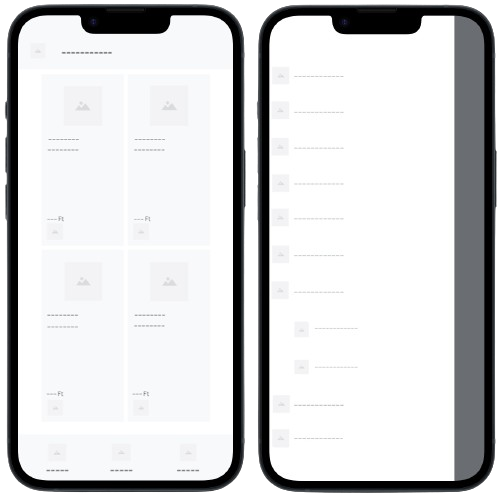
\includegraphics[width=0.3\linewidth]{img/ui_mockup.png}
	\caption{Mobile User Interface Mock-up}
	\label{fig:ur5}
\end{figure}

\subsection{Technological Stack}

The final product's overall success is largely dependent on the technological choices made during the project. A modern, flexible, and extremely efficient application can be developed by selecting a technology stack that includes MongoDB, ASP.NET, Angular, and .NET MAUI. When these technologies are combined, they form a strong and stable foundation that significantly raises the chances of project success. Each technology has advantages of its own.

\textbf{MongoDB} is a highly flexible and scalable data management system created especially for contemporary web applications is called {MongoDB}. Because it is a NoSQL database, it excels at managing dynamic data requirements, which makes it a great option for companies that operate in the fast-paced digital world of today. MongoDB manages enormous volumes of data with ease and is able to quickly adjust to changing data schemas thanks to its document-oriented architecture. Because of its remarkable flexibility, businesses can easily adapt their data models to the demands of their industries and quickly change their business requirements. Furthermore, the database can readily expand as the project grows thanks to MongoDB's built-in scalability and cloud-based deployment features, guaranteeing seamless performance and ideal data storage.

\textbf{ASP.NET API} is a powerful, incredibly secure framework with outstanding performance, which makes it a great option for creating enterprise applications. Developers can quickly and simply construct a dependable, orderly backend system that effectively manages a variety of client-side requests by using the ASP.NET API. Modern web applications can be built with the framework because of its built-in security features, which include support for RESTful APIs, optimization capabilities, and authentication and authorization.

\textbf{Angular} is a popular JavaScript framework created especially for making dynamic and interactive web applications. This adaptable framework gives developers a strong tool to quickly and effectively create user-friendly and responsive interfaces. It is made to function flawlessly across many platforms. With Angular's extensive feature set, which includes data binding, modular development, and testing capabilities, you can create beautiful, user-friendly websites that are both aesthetically pleasing and easy to maintain.

With the release of \textbf{.NET MAUI} by Microsoft, a cutting-edge framework created especially for cross-platform mobile application development is introduced. Using a single code base, developers can create top-notch apps for Windows, iOS, and Android platforms with this state-of-the-art framework. Developers can leverage the same code across platforms with.NET MAUI, saving a lot of money and time while still taking advantage of the distinct features and interfaces offered by each native operating system.




\clearpage
\section{IMPLEMENTATION}
\subsection{Introduction}

In this crucial section of my thesis, I explore the pragmatic aspects of the implementation process, revealing the manner in which my proposed solution was actualized. The proposed solution incorporates a comprehensive system consisting of four essential components: a MongoDB database, an ASP.NET API, an Angular web application designed for administrative purposes, and a .NET MAUI mobile application that is compatible with both iPhone and Android devices. The purpose of this section is to offer a comprehensive explanation of each module, elucidating their respective contributions to the overall software solution.

Each upcoming section contains different parts of my solution, starting with stating the reason why I chose each technology for that specific part. Discussions on why MongoDB was chosen as the database, the benefits of using ASP.NET to create the API, the choice of Angular for the web app, and the advantages of using.NET MAUI to create cross-platform mobile apps have been included. The evaluation is not only about the choice, but also about how these technologies work together to make a system that works as a whole.

I will also carefully look over all the details of the implementation process. This includes the structure and architecture of each module, the design patterns that were used (if any), and the addition of different frameworks and libraries that made the system work better and be more useful. This section will not only explain these parts, but will also include code examples to help you understand how they work in a clear and useful way.

Dealing with the different problems and challenges that come up along the way is an important part of this project. In this part of my thesis, I want to talk about the problems I faced personally when trying to solve these problems, the plans I made to get past them, and the insights I gained from these experiences. These thoughts are meant to give a realistic picture of the implementation process, focusing on both its successes and problems.

In summary, this section will focus on the practical aspects of my thesis, specifically the implementation of certain components, their interplay, encountered challenges, acquired experiences, and the strategies employed to address said issues.

\subsection{Database}

\subsubsection{Introduction}

With the quick rate of technological progress and digital change, the massive volume of data on the Internet can sometimes appear overwhelming and chaotic. Effective handling of this complicated, frequently badly structured, and abundant data is critical. MongoDB is a NoSQL database that varies from typical relational databases. It is appropriate for dynamic, changing situations, since it can manage massive volumes of data and is flexible enough to swiftly react to changes.

In my situation, MongoDB was an ideal choice for the solution because maintaining an extensive amount of shop item data and the necessity for quick queries required the use of a technology like such. In this section, I will highlight the primary benefits of MongoDB to justify its use, and then show how the database and its collections were configured for the solution.

\noindent\textbf{Why MongoDB} 

\textbf{Flexibility and Scalability:} The schema-less nature provides enormous flexibility, allowing for the easy integration of diverse and growing data formats. This helps with shop item data, which may have multiple properties. MongoDB's horizontal scalability can handle massive datasets, ensuring database performance as shop items increase. It may come in handy in case different types of data will need to be stored in the same database.

\textbf{Performance and Efficiency:} The document-oriented structure allows for swifter read/write operations. This is critical for e-commerce platforms, as quick data retrieval and updates for store products are critical for user experience and operational efficiency. The adoption of the BSON (Binary JSON) format improves efficiency even more, especially for sophisticated queries across big datasets.

\textbf{Agile Data Handling:} The dynamic query language in MongoDB is a powerful tool for quickly working with data and managing inventory in retail settings. It can handle many different types of data, which makes it perfect for e-commerce. It also lets you do complex queries like text searches, real-time aggregation, and range queries. This feature is very important for sorting, filtering, and analyzing products based on things like price, category, and availability. MongoDB is also very important for managing the connections between different types of data, which makes it easier to get a full picture of inventory. Businesses can quickly respond to changes in the market, as well as to customer wants with this unified approach. It also helps with organization and making smart product management decisions. 

\newpage

\textbf{Driver Support:} The platform offers official drivers and libraries for widely used programming languages, including Python, Java, C\# and Node.js. 
I connected the ASP.NET API to MongoDB using the official driver to store and retrieve data efficiently. MongoDB also has extensive documentation and a vibrant community to help integrate it into various technological environments. 
\newline \cite{mongodb}

\subsubsection{Database Structure}

Although MongoDB was not explicitly designed with focus on handling relational data, it is still capable of managing relationships between data entities. Entity Relationship Diagrams (ERDs) were employed to depict the entities within the collections, aiming to provide a more comprehensive and easily understandable illustration of their relationships. 
Within the database, there exist several collections, namely "users", "admins", "shop-items", "categories", "sub-categories", and "shops". In the following part, a detailed description will be provided regarding the different characteristics of each entity.

\noindent\textbf{User Data:} 

Users' basic information and associated session data are both included in the users collection. The entities in the admins collection have foreign keys pointing to particular user entities. Users and the admins collection have a zero-to-one relationship because not every user has administrative privileges. In this case, the role field indicates the user's assigned role; it does not necessarily imply that the user has administrative privileges unless the user is specifically linked to an administrative entity. The configuration described above simulates a real-world scenario where only particular users have administrative privileges. The depicted structure is observable on figure \ref{fig:uerd} provided below.

\begin{figure}[H]
	\centering
	\includegraphics[width=0.36\linewidth]{img/Users_erd.png}
	\caption{Entity Relationship Diagram of User Data}
	\label{fig:uerd}
\end{figure}

\noindent\textbf{Shop Item Data:}

Collections are responsible for managing the hierarchical structure of shop items, which is organized into categories and sub-categories. Every item in a shop is linked to a particular category and possibly a sub-category, which aids in the systematic retrieval of data and the effective categorization of products.

The collection of shop-items, which serves as the core component of the database, encompasses comprehensive data pertaining to each individual item. This data includes references to the item's category, sub-category, and the specific shop to which it is affiliated. The shop entity contains information pertaining to each individual shop or vendor. The establishment of this relationship is crucial in effectively managing the inventory and gaining valuable insights into the range of products offered by each individual shop. The structure is visualized on figure \ref{fig:serd} below.

\begin{figure}[H]
	\centering
	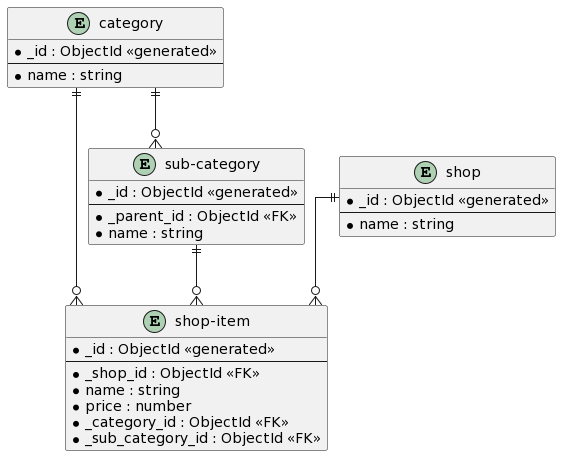
\includegraphics[width=0.85\linewidth]{img/shop_items_erd.png}
	\caption{Entity Relationship Diagram of Shop Item Data}
	\label{fig:serd}
\end{figure}

In conclusion, for large shop item data, MongoDB is flexible, fast, and scalable. The database schema meets the complex relationships between users, admins, categories, subcategories, shop items, and shops. It handles large amounts of data efficiently and adapts to e-commerce platforms. Thus, MongoDB is ideal for modern data management, especially for large, multifaceted datasets like shop items.

\newpage

\subsection{Application Programming Interface}

\subsubsection{Introduction}

When making modern software, the technology you use to build an Application Programming Interface (API) is very important. I chose to use ASP.NET Core along with the programming language C\# for the API part of my project. Several important factors, each of which added to the overall efficiency and reliability of the API, led to this decision.

One of the main reasons for choosing ASP.NET Core is its ability works well with many NuGet packages. NuGet packages are basically code libraries or tools that are easy to add to a project. They provide a huge collection of resources that can improve functionality and speed up development. This wide range not only speeds up the development process but also gives you access to a lot of pre-built features, so you don't have to start from scratch.

Another big plus is that ASP.NET Core works natively with the Internet Information Services (IIS) server. This integration makes deployment and hosting easier, which guarantees strong performance and dependability. Its compatibility with MongoDB's driver makes it even more appealing, as it makes database interactions faster. Also, the fact that this framework has libraries for web scraping makes it easy to get data from different web sources, which is exactly what the project needs.
\newline\cite{aspnet}

The solution is designed so that the API is the central part of the application. It provides several features, like asynchronous web scraping, data manipulation, and providing important endpoints for both the web and mobile parts of the system. Also, it's an important security layer that handles how the applications and the database talk to each other, keeping the data safe and secure.

The authentication and authorization processes that the API handles add to the security by making sure that access to data and features is tightly controlled and in line with best practices. The Model-View-Controller (MVC) design pattern, which divides an app into three parts that are all connected, forms the basis of the API's structure. This not only makes the code cleaner and easier to maintain, but it also helps separate concerns, which makes the system more modular and scalable.

One interesting thing about the API is that it uses OpenAI to process and organize data that it gets from web scraping. As a result of this integration, the API can do more than just handle data. It's an innovative combination of traditional web development methods and artificial intelligence technologies.

\newpage

To sum up, the decision to use ASP.NET Core with C\# for the API is a smart move that takes advantage of a strong, flexible, and effective technology stack. It's made to handle the application's complicated needs, giving a solid base for working with data, keeping it safe, and making it easy to connect to other parts of the system.

\noindent\textbf{Structure of the API}

\subsubsection{Entry Point}

The setup process revolves around \textbf{WebApplicationBuilder}. This builder lets developers configure app services and settings. CORS policies instruct the web app how to handle requests from different domains. This is crucial for modern web apps that use resources or APIs from different domains to ensure safety and functionality. Configuration includes database service setup. User model, shop item, shop item category, and shop scraping services are added as singletons, meaning they are used once throughout the application.

The code also configures JWT authentication. This is crucial to modern web apps because it restricts access to resources and endpoints to verified users. This app uses these tokens to verify users' identities and manage them well, such as by getting them from cookies.

The final step is building the app and setting up its middleware pipeline. This pipeline manages HTTP requests, CORS, authentication, and controller requests. Controllers require a RESTful API design with multiple endpoints for different web requests. After saving the settings, the app can be launched and serve requests as a web server.

\subsubsection{Controller}

The \textbf{DataBaseService} is an important part of the proposed system architecture. It acts as a flexible data service with generic datatype of for the model. This helps with the developer as creating a new controller is relatively easy, promoting high flexibility for future changes. It manages the flow of information between the controllers and the MongoDB driver.  

The ASP.NET Core \textbf{ControllerBase} class is at the heart of this structure, and an ApiControllerBase class is carefully built on top of it. Its design is naturally generic, which makes it useful because it can be used as a base for building different kinds of controllers that are each made to work with specific models, therefore promoting scalability.

In addition to managing a lot of asynchronous methods related to data manipulation, this derived class is also in charge of managing JWT tokens within cookies crucial to the security of the endpoints. The 'AllowAnonymous' attribute on the HTTP method in the derived controller can selectively bypass JWT authentication.

The architecture also includes the \textbf{ShopItemController} and \textbf{ShopItemCategoryController}, which are both used to change the general properties of their own data types. This controller is used by, the mobile application to retrieve data and the scraping service to expand, update the data warehouse.

The \textbf{UserController} is the most complicated of these. Its job is to handle a wide range of user-related tasks. These include creating and deleting user accounts, logging in and out, authenticating users, verification of administrative privileges, assigning admin rights, and renewing refresh tokens that have expired.

Shown below is a detailed class diagram, so that one can fully understand how the different parts of this system work together. Figure \ref{fig:ccd} shows very clearly how different classes and interfaces are linked to each other, along with their properties and methods.

\begin{figure}[H]
	\centering
	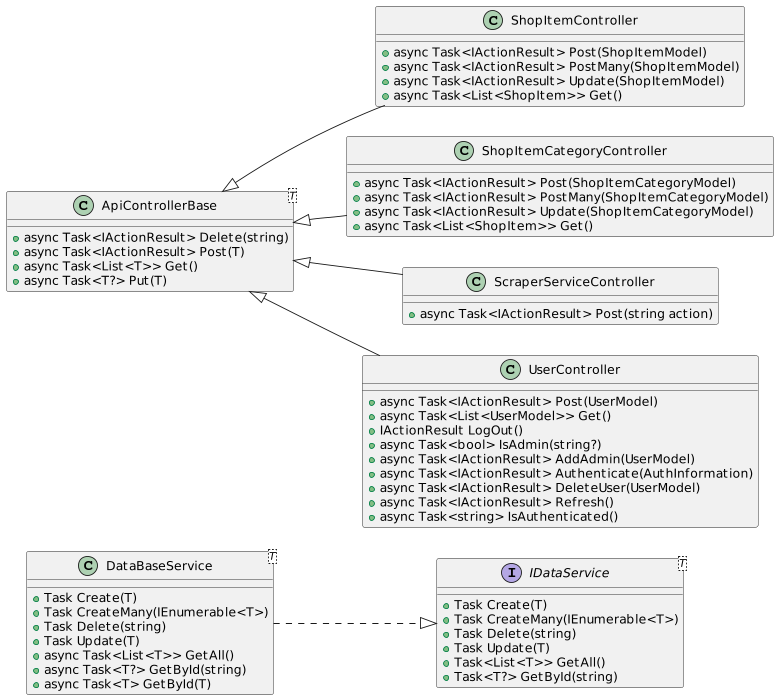
\includegraphics[width=1\linewidth]{img/controller_classdiagram.png}
	\caption{Class Diagrams Related to the Controller}
	\label{fig:ccd}
\end{figure}

\newpage

\noindent\textbf{UserController in Detail}

Since UserController is a complex part of the application, mostly because that is how it handles authentication, it is useful to talk about the implementation in detail.

\begin{algorithm}
	\caption{Refresh Access Token}
	\begin{algorithmic}
		\State Initialize principal from expired token
		\State $userName \gets$ principal.Identity.Name
		\State $user \gets$ databaseService.Get(userName)
		
		\If{$user = \text{null} \lor user.RefreshToken = \text{null} \lor user.RefreshTokenExpiryTime < \text{DateTime.Now}$}
		\State \Return BadRequest()
		\EndIf
		
		\State $newAccessToken \gets$ jwtAuthenticationManager.GenerateAccessToken(principal.Claims)

		\State Response.Cookies.Append(Constants.AccessToken, newAccessToken)
		
		\State \Return Ok()
	\end{algorithmic}
\end{algorithm}

Visible on the algorithm above, an interesting part of the authentication process is the JWT refreshing. Since the Access Token's lifespan is only a few seconds (security reasons), most of the requests require refreshing this token on the server-side with the request principal, setting the user's cookie before fulfilling the request.

Upon registering, the user's provided password is immediately hashed and only stored afterwards, and in every login process the hashed passwords are being matched to each other.
On logging out, the system removes all the cookies from the user, which is achieved by setting the cookies expiration date to a value, which will essentially turn them invalid.

Regarding the addition of a new admin user, the process will only be successful when the user assigning admin role to another user has admin privileges. More on the authentication process, with detailing the JWT authentication process will be discussed in the next section.

\subsubsection{JWT Authentication}

The authentication for the web uses JSON Web Tokens and takes advantage of AspNetCore's Authentication library, as well as the IdentityModels's Jwt token library. JSON Web Tokens (JWTs) are compact, URL-safe claims that are used for secure authentication and information exchange in web applications. \cite{jwt}

Figure \ref{fig:acd} represents the class for holding authentication information, as well as the authentication manager class, which is responsible for handling all JWT authentication related tasks, described using pseudo code.

\begin{figure}[H]
	\centering
	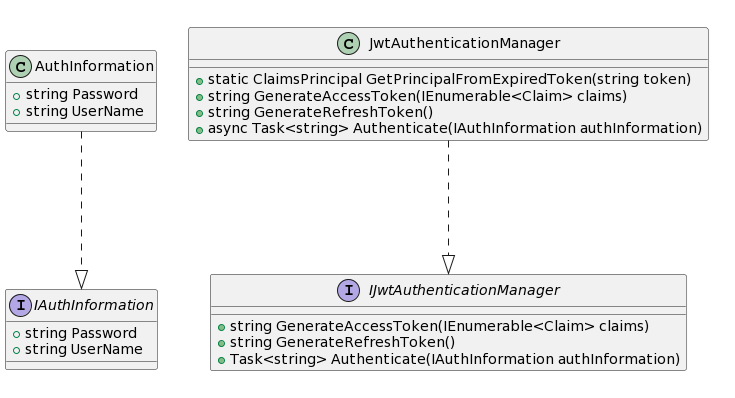
\includegraphics[width=0.7\linewidth]{img/authentication_classdiagram.png}
	\caption{Class Diagrams Related to JWT Authentication}
	\label{fig:acd}
\end{figure}

\begin{algorithm}
	\caption{Authentication Manager}
	\begin{algorithmic}
		
		\Function{GetPrincipalFromExpiredToken}{token}
		\State Validate JWT with tokenValidationParameters
		\If{securityToken is HMAC SHA256}
		\State \Return principal
		\Else
		\State Throw new SecurityTokenException
		\EndIf
		\EndFunction
		
		\Function{GenerateAccessToken}{claims}
		\State Convert key to byte array
		\State Setup tokenDescriptor with claims and signing credentials
		\State Create token using tokenDescriptor
		\State \Return token
		\EndFunction
		
		\Function{GenerateRefreshToken}{}
		\State Returns a random32-byte buffer as Base64 string
		\EndFunction
		
		
		\Function{Authenticate}{authInfo}
		\If{username and password combination is valid}
		\State Create new claims for user
		\State Generate and \Return access token
		\Else
		\State \Return empty string
		\EndIf
		\EndFunction
		
		
	\end{algorithmic}
\end{algorithm}
 
\subsubsection{Data Models}

While being an essential part of the MVC pattern, the  data models in the application are mostly used for data representation, and moving data in a structured way between the API endpoints and the database. Only the UserModel includes specific methods for password hashing and verifying using \textbf{BCrypt.Net-Next library's} \textit{EnhancedVerify()} method, that checks a plaintext password against a hashed version to ensure secure authentication, as well as \textit{EnhancedHashPassword()} method, that uses bcrypt hashing algorithm and other security enhancements to make storing passwords secure. The structure of the data models used by the controllers as well as showcasing how easily extensible the genereic controller implementation is shown on the figure \ref{fig:dcd}.

\begin{figure}[H]
	\centering
	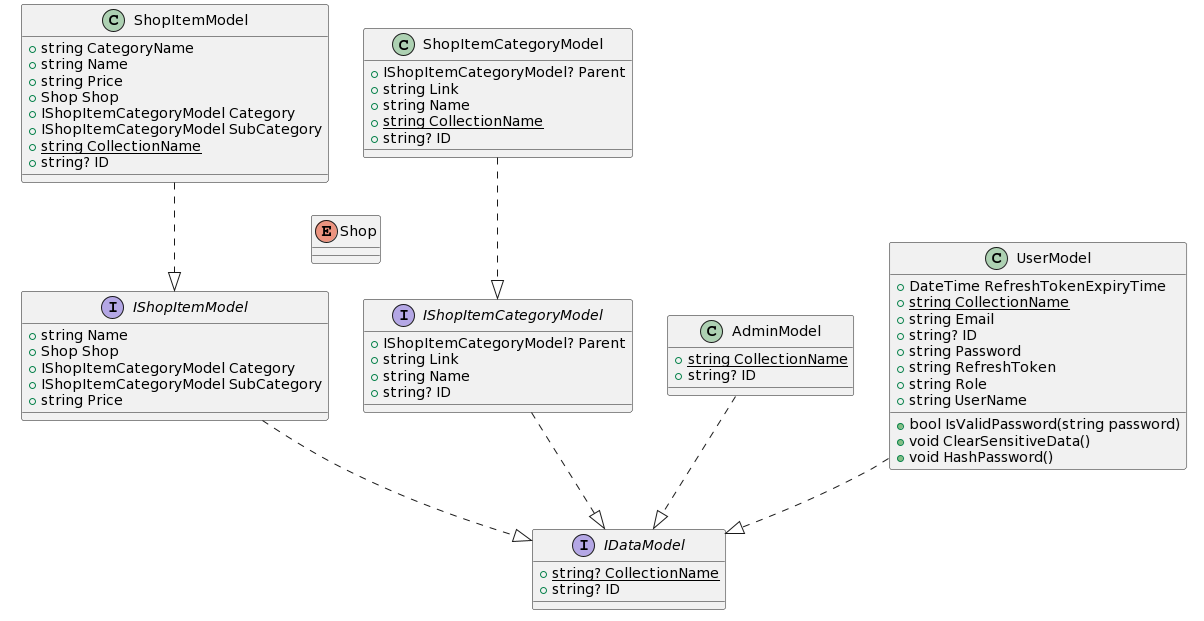
\includegraphics[width=1\linewidth]{img/datamodel_classdiagram.png}
	\caption{Class Diagrams Related to Data Models}
	\label{fig:dcd}
\end{figure}

\newpage

\subsubsection{Web Scraping}
In the solution the API is responsible for handling the data collection from the web as well. The scraping service is accessible from the website on a specific page available for administrators only, where they can force an immediate process or set a time interval for automatic executions. For crawling the web, the solution uses a version of Selenium framework provided for .Net applications.

Selenium is a free and open-source automation tool that is mostly used to automate web browsers. It gives engineers a solid way to check web applications. Many people choose Selenium for cross-browser automation for it has many useful parts, such as Selenium WebDriver for managing how browsers work, which is crucial in this case.

The first approach consisted of downloading the page's HTML code, however, it turned out, that nowadays most of the websites load content dynamically, so the data downloaded was of no use. To overcome this, the application uses Selenium for simulating a head-less browser, which is a web browser that doesn't have a graphical user interface. It lets programs control web pages automatically, which is why it's often used for web scraping, automated testing, and rendering web pages for processing on the server.

Scraping also states an issue with protection of the site's data. The general rule is that you are only supposed to collect data that you can publicly access and if the site's robots.txt file content does not prohibit you from scraping the data available on the website. Before crawling a new website for data, it is essential to review these points.

Shown below on figure \ref{fig:scd} are the classes and interfaces that are required for the service to work, the characteristics of its working process are explained on the next page.

\begin{figure}[H]
	\centering
	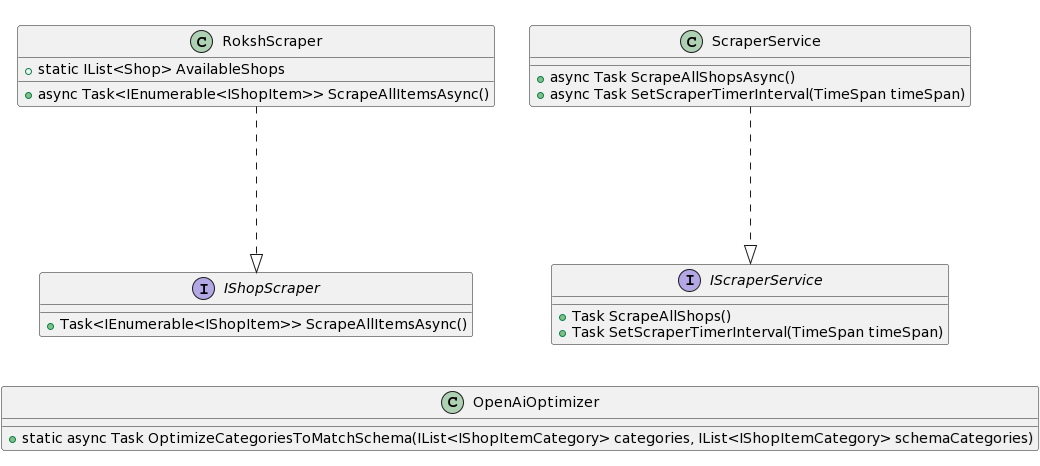
\includegraphics[width=1\linewidth]{img/scraping_classdiagram.png}
	\caption{Class Diagrams Related to Web Scraping}
	\label{fig:scd}
\end{figure}

\noindent\textbf{How Does It Scrape}

First of all, the ScraperService is exported as a singleton IScraperService during the application setup process. The ScrapeServiceEndpoint listens for post requests, and upon a valid request takes action. It is configured to allow requests for immediate and timed scrapings. 

Before scraping, the service configures the parameters for the WebDriver and calls for all of the available IShopScraper implementations. Since many websites differ in their structure, most of them need separate implementations to specify what instructions are required for the data retrieval. 

After finishing the setup, the service starts all of the IShopScrapers data collection processes on different threads to speed up the process, then waits for all of them to finish. On finishing it checks the integrity of the data, using fuzzy string matching and uploads the data into the database.

The process of scraping the items from various websites always needs fine tuning, but roughly follows the same idea implementing HTML and CSS tag verification, which will be presented with the following four pseudo-like algorithm descriptions.


\noindent\textbf{ScrapeAllItemsAsync Method} is the one being called from the Service and in the end provides structured shop item data with correct categories provided by the application.

\noindent\textbf{GetCategoriesWithSubcategories Method} is the one responsible for mapping all categories and subcategories on the site with storing their links to easily load when needed.

\noindent\textbf{ScrapeShopItemsAsync Method} visits every subcategory and scrapes all the items that are available on that page, then stores them for later use.

\noindent\textbf{ScrollTillEnd Method} is crucial for the scraping process, since it handles the scrolling and waiting process, to make sure that the dynamically loading item data is present and scrapable.

\begin{algorithm}
	\caption{ScrapeAllItemsAsync Method}
	\begin{algorithmic}
		\State $attempts \gets 0$
		\State $maxAttempts \gets 3$
		\While{$attempts < maxAttempts$}
		\State \textbf{try to}:
		\State \hspace{\algorithmicindent} $items \gets \text{ScrapeShopItemsAsync().ToList()}$
		\State \hspace{\algorithmicindent} $\text{webDriver.Quit()}$
		\State \hspace{\algorithmicindent}\hspace{\algorithmicindent} $\text{OpenAiOptimizer.}$
		\Statex \hspace{\algorithmicindent}\hspace{\algorithmicindent} \hspace{\algorithmicindent} $\text{OptimizeCategoriesToMatchSchema(allCategories, defaultCategories)}$
		\State \hspace{\algorithmicindent} \Return $items$
		\State \textbf{if} exception occurs \textbf{then}
		\State \hspace{\algorithmicindent} $attempts \gets attempts + 1$
		\State \hspace{\algorithmicindent} \textbf{if} $attempts > maxAttempts$ \textbf{then}
		\State \hspace{\algorithmicindent}\hspace{\algorithmicindent} Print exception $e$
		\State \hspace{\algorithmicindent}\hspace{\algorithmicindent} \textbf{break}
		\EndWhile
		\newline
		\Return new list of IShopItem
	\end{algorithmic}
\end{algorithm}

\vspace{-500pt}

\begin{algorithm}
	\caption{GetCategoriesWithSubcategories Method}
	\begin{algorithmic}
		\State Initialize dictionary $categoriesWithSubCategories$
		\State Create a new WebDriverWait with 5 seconds timeout
		\For{each category element found by webDriver}
		\State Click on the category element
		\State Create a ShopItemCategory
		\State Initialize list for $subCategories$
		\For{each subCategory in the category element's parent}
		\State Add new ShopItemCategory to $subCategories$
		\EndFor
		\If{no $subCategories$}
		\State Add the main category as a subcategory
		\EndIf
		\State Add category and its $subCategories$ to the dictionary
		\EndFor
		\newline
		\Return dictionary
	\end{algorithmic}
\end{algorithm}

\begin{algorithm}
	\caption{ScrapeShopItemsAsync Method}
	\begin{algorithmic}
		\State Navigate webDriver to URL
		\State Initialize list of IShopItem $items$
		\For{each category in GetCategoriesWithSubcategories}
		\For{each subCategory in category's value}
		\State Add $subCategory$ to allCategories
		\State Navigate webDriver to $subCategory$'s link
		\State Call ScrollTillEnd
		\For{each item found by webDriver}
		\State Create and add new ShopItem to $items$
		\EndFor
		\EndFor
		\EndFor
		\newline
		\Return $items$
	\end{algorithmic}
\end{algorithm}

\begin{algorithm}
	\caption{ScrollTillEnd Method}
	\begin{algorithmic}
		\State Initialize $endOfPage \gets false$
		\State Create a new WebDriverWait with 5 seconds timeout
		\While{not $endOfPage$}
		\State Get count of items found by webDriver
		\State Scroll to the end of the page
		\State \textbf{try to}:
		\State \hspace{\algorithmicindent} Wait until more items are found
		\State \textbf{if} exception occurs \textbf{then}
		\State \hspace{\algorithmicindent} Set $endOfPage \gets true$
		\EndWhile
	\end{algorithmic}
\end{algorithm}

\newpage

\subsubsection{OpenAI Processing}

Unfortunately it can't be guaranteed that each site has the same categories for the products listed, therefore I needed a solution to match these. Fuzzy string matching would not be reliable enough, therefore I turned to OpenAI's chat endpoint and utilized it the following way: Before returning the data to the ScrapingService, the IShopScraper calls of the OpenAiOptimizer's OptimizeCategoriesToMatchSchema method.

A system calls the OptimizeCategoriesToMatchSchema method to divide categories into 10 groups and asynchronously send them to OpenAI's ChatGPT as JSON data. ChatGPT matches these categories to a schema and returns renamed JSON categories. After renaming the categories, the method returns the modified data to the calling system. This way AI-driven classification and automated data processing are also shown in this web application.

Interesting remark about the prompting process, is that it is not included in a ChatGPT subscription, instead it uses a credit / prompt system, which has become much cheaper since the introduction of the GPT 3.5 turbo model. The code also needs to be prepared for occasional outages, when it needs to retry the prompt. Writing a message with instructions for ChatGPT can be challenging too, I overcame this by writing a sturdy prompt message and asking ChatGPT to reply with a JSON format of the data. This sometimes also produced extra message and characters around the JSON format, which I worked around by trimming all the characters, outside the JSON body format. On figure \ref{fig:ai} a simplified version of the process is shown via sequence diagram.

\begin{figure}[H]
	\centering
	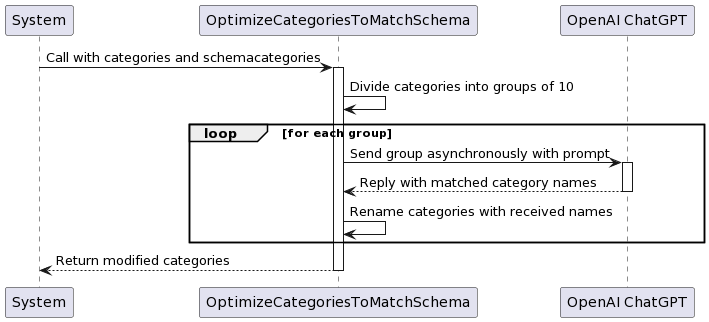
\includegraphics[width=1\linewidth]{img/openai_sequence.png}
	\caption{Open AI Category Aligning Sequence Diagram}
	\label{fig:ai}
\end{figure}

\pagebreak

\subsection{Web Application}

\noindent\textbf{Who is it for?} It is very important to note, that the web application is solely for administration purposes and will only be accessible by the program's administrators and the associated retailers to provide them a way to upload their product data. In this section by users I essentially mean one of the retailers who are providing data for the application.

\subsubsection{Introduction}

As the framework of choice for this app, Angular was chosen, because it has a large ecosystem and a lot of strong features that make it perfect for a modern, dynamic web app.

As a platform known for its structured framework and wide range of tools, Angular makes it easy to build large-scale apps with its opinionated architecture. This prescriptive nature makes it much easier to keep codebases consistent, which makes it perfect for the application's complicated structure, which needs clear modularity and separation of concerns.

Angular's powerful typing system, which is powered by TypeScript, makes code better and more reliable. This makes debugging and maintenance easier, which is important for the long-term growth and scalability of the app. Using reactive programming patterns with RxJS also makes it easier to work with asynchronous data streams, which are needed for the app's real-time data processing features like uploading product data and scraping the web.

Built-in features of the framework, like dependency injection, routing, and services, make it easier to make applications that are safe and work well. The app uses these features to keep track of user authentication states, protect routes based on user roles, block HTTP requests, and easily talk to back-end services. Moreover, the architecture carefully arranges how users interact with it, how it is protected, and how it handles data through a clear set of modules.
\newline\cite{angular}

By implementing SSL certificates for the web page and API, the application enables HTTPS protocol and ensures secure communication. Sensitive data, including passwords and tokens, is protected by this configuration, which encrypts data transferred between the server and client. By using HTTPS instead of HTTP, users can be assured that their data is encrypted and unintelligible even if it is intercepted, creating a secure and reliable environment. The application's design is based on this commitment to security, and it fits in perfectly with Angular's framework, which facilitates strong security implementations.

\newpage

\subsubsection{Architecture}

The following diagram, visible on figure \ref{fig:webappstruct} makes it easy to see how the application is structured. Every module makes sure that the user has a safe, quick, and smooth experience by explaining its function in the application and how it works with the other modules. This organized method makes things run smoother and sets the stage for future improvements.

\begin{figure}[H]
	\centering
	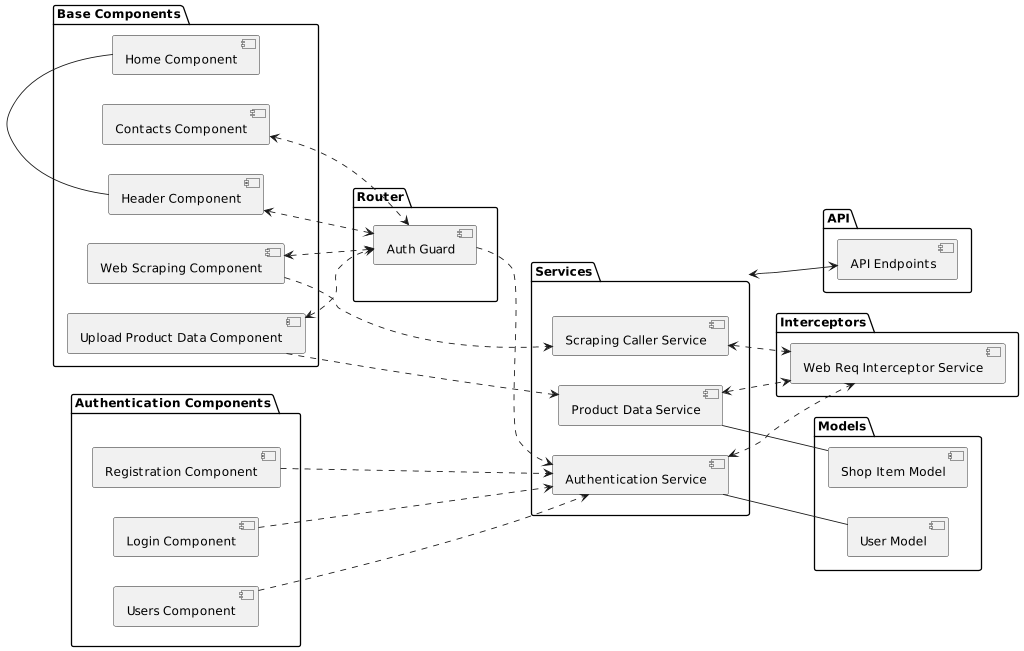
\includegraphics[width=1\linewidth]{img/website_structure.png}
	\caption{Structure of the Web Application}
	\label{fig:webappstruct}
\end{figure}

\noindent\textbf{Base Components: }

The Base Components make up the main part of the user interface. The Home Component is a landing page with useful information that all visitors can see. The Header Component goes with it and makes sure that the application's navigation and branding are all the same. The header navigation depends on whether a user is authenticated or not as well as if they have admin privileges or not. 

\noindent\textbf{Authentication Components:}

It essentially includes two main parts: the Registration Component, which lets new users create accounts, and the Login Component, which helps users prove who they are. Both parts are necessary to start the user's journey within the app by giving them JWT access and refresh tokens when they successfully register or login.

On figure \ref{fig:auth} the UI of the two authentication components, login and registration functionalities are visible. 

\begin{figure}[H]
	\centering
	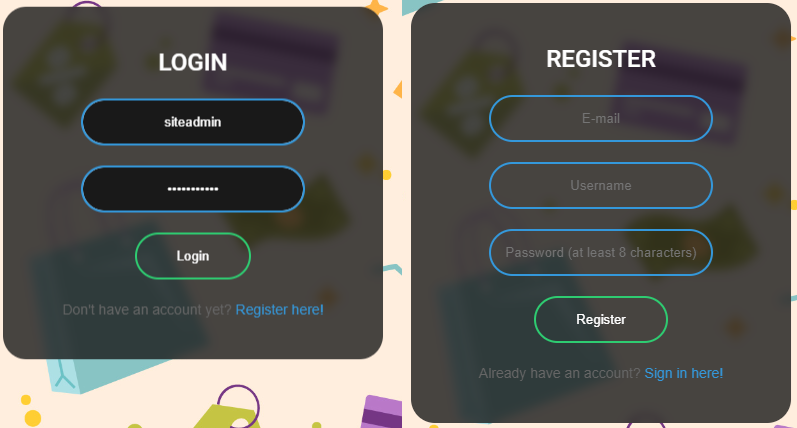
\includegraphics[width=0.7\linewidth]{img/auth_web_ss.png}
	\caption{Authentication on the Website}
	\label{fig:auth}
\end{figure}

\noindent\textbf{Specialized Access:}

Two essential components—the Web Scraping Component and the Users Component—are only accessible to admin users. With the former, administrators can set up and start web scraping activities on demand or at predetermined intervals, which functions are provided with an easy to use user interface shown on figure\ref{fig:webcrapingreq}.
\begin{figure}[H]
	\centering
	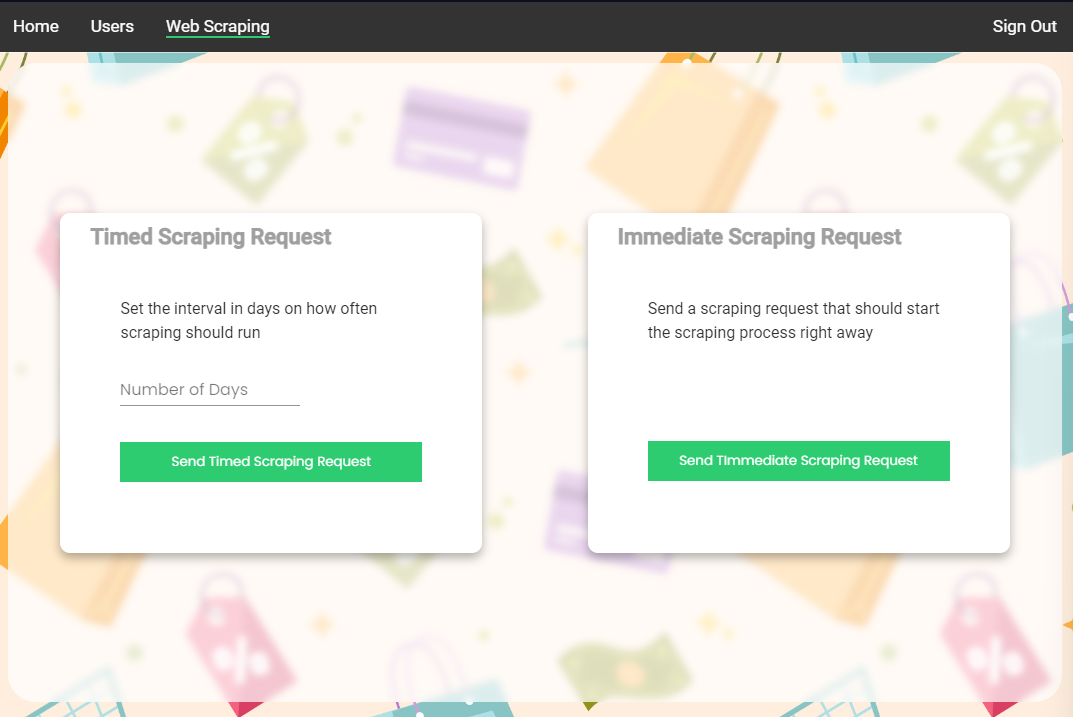
\includegraphics[width=0.9\linewidth]{img/scraping_web_ss.png}
	\caption{Requesting Web Scraping}
	\label{fig:webcrapingreq}
\end{figure}

\newpage

With utilizing the Users Component, the administrators can view a complete list of users available for the web application, change their permissions within the application or completely remove them from the list. The interface for these functions are shown on figure \ref{fig:umgmt} below.

\begin{figure}[H]
	\centering
	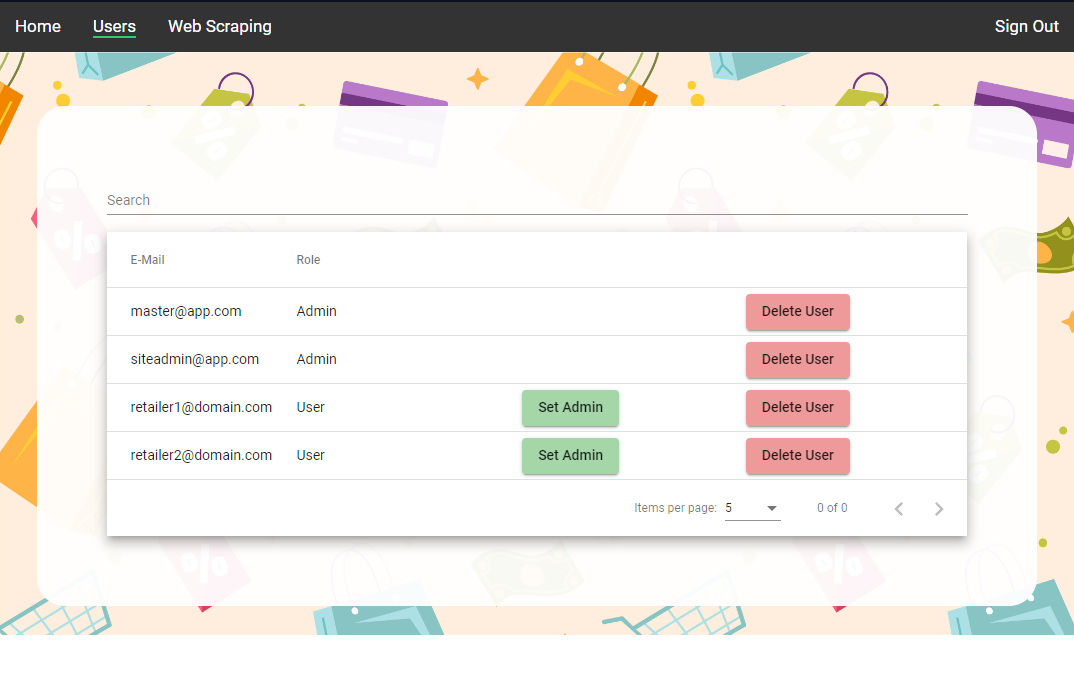
\includegraphics[width=0.8\linewidth]{img/users_ss.png}
	\caption{Web Application's User Management}
	\label{fig:umgmt}
\end{figure}

\noindent\textbf{User-Focused Functionality:}

Authorized users are given permission to access the Contacts Component for the purpose of communication, and the Upload Product Data Component. The latter component, shown on figure \ref{fig:uploaddata} is provided for users to upload product data, which is then processed by the Product Data Service, which converts CSV inputs into JSON format and checks that they match the Shop Item Model before submitting them to the API.

\begin{figure}[H]
	\centering
	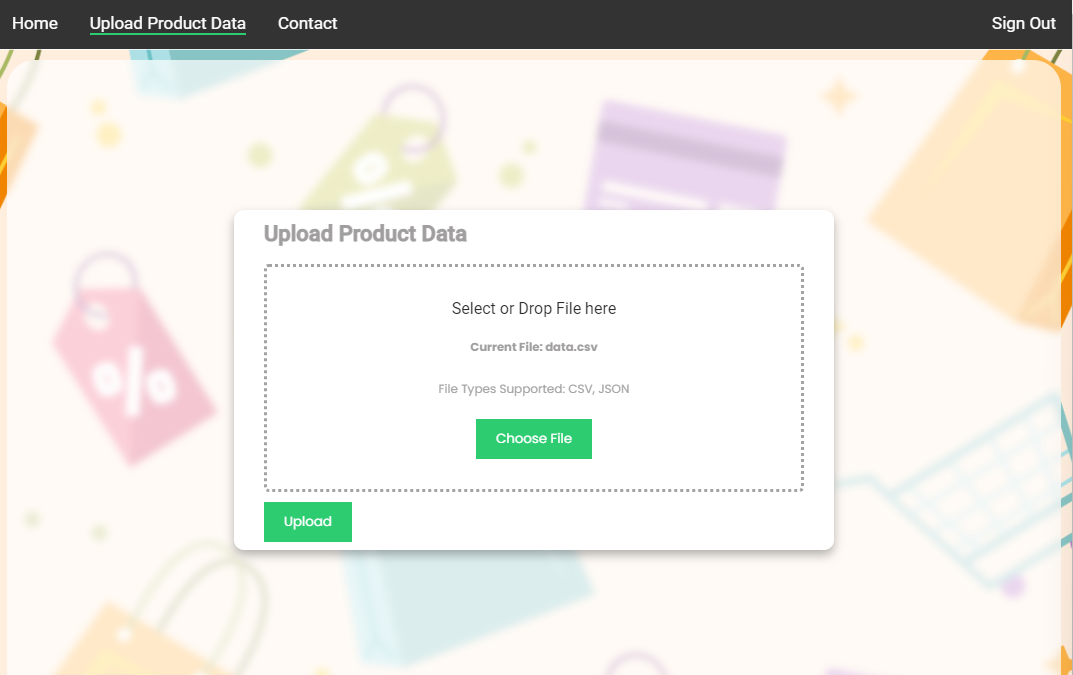
\includegraphics[width=0.65\linewidth]{img/product_data_ss.png}
	\caption{Upload Product Data}
	\label{fig:uploaddata}
\end{figure}

\noindent\textbf{Services:} 

The logic of the application is contained within the Services, which includes the Product Data Service, Authentication Service, and Scraping Caller Service. To fulfill specific application functionalities, each service interacts with the corresponding components and API Endpoints.

\noindent\textbf{Data Models:} 

The User Model and the Shop Item Model define the structure for user information and product data. These models are critical for the application's data integrity and consistency.

\noindent\textbf{Interceptors:} 

All outgoing requests are carefully watched over by the Web Req Interceptor Service. It makes sure that authentication keeps going by refreshing tokens (visible on figure \ref{fig:cookies}) through the Authentication Service when needed and stopping requests and logging out the user if serious problems are found.

\begin{figure}[H]
	\centering
	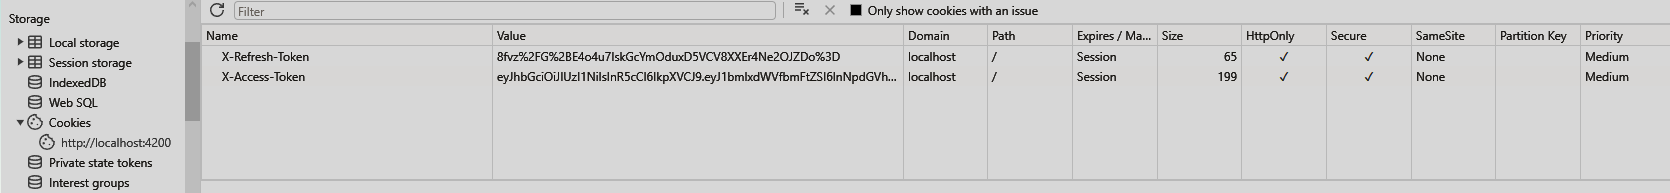
\includegraphics[width=1\linewidth]{img/cookies_ss.png}
	\caption{JWT Tokens Stored in Cookies}
	\label{fig:cookies}
\end{figure}


\noindent\textbf{Router:} 

The Router and Auth Guard are essential to the application's security architecture. It ensures that non-authenticated users can only access the Home, Registration, and Login Components by clearly defining user interfaces and component accessibility. Admins and verified users, on the other hand, have access to extra, role-specific features.

\noindent\textbf{API Communication:}

Backend interaction happens through the API package. The document defines the endpoints that the application uses to talk to the backend, trusting the Services to do all of those tasks efficiently.

\noindent\textbf{Ending Note:}

Even though the web application only serves administrative purposes, it was still important to provide this functionality in a user friendly manner. From development side, since the future is malleable, choosing Angular was the right way to ensure modularity and scalability. 

\newpage

\subsection{Mobile Application}

\subsubsection{Introduction}

The following chapter of this thesis discusses the mobile application I created using the .NET MAUI framework. .NET MAUI is a modern cross-platform development tool that enables applications to be easily adapted to a variety of operating systems, including Android, iOS, TizenOS, and macOS. I used several NuGet packages during the application's development, which significantly increased functionality and user experience. These packages include CommunityToolkit.Maui, which supports specific user interface elements, FuzzySharp, which enables fuzzy search based on product names, and ZXing.Net.Maui, which helps with barcode reading and decoding.

During the project's development, I used the MVVM (Model-View-ViewModel) design pattern, which is a common architectural pattern in modern application development. The benefit of MVVM is that it effectively separates the user interface (View), data model (Model), and presentation logic (ViewModel). This separation simplifies the development process by allowing components to be tested and maintained more easily. The ViewModel serves as an intermediary between the model and the view, reducing direct dependencies and increasing the application's flexibility, making it easier for developers to manage business logic and user interface.
\newline\cite{maui}

The current application can be compared to a Minimum Viable Product (MVP), as it demonstrates basic functionality and serves as a solid foundation for future development. The MVP approach allows for the collection of user feedback in the early stages of a project, which can then be used to better determine future development directions. The scope of the project is extensive, and many ideas have yet to be implemented. In the field of software development, it is common to adapt and redesign in comparison to the original plans, which is difficult, but the MVP approach used allows the application to gradually develop further, achieving a balance between user needs and project framework. \cite{mvp}

In the following sections, I will discuss the architecture of the application, the persistence of data, I will highlight some interesting solutions that have been implemented, and I will provide an overall general idea of how the application functions.

\pagebreak

\subsubsection{Service Layer}

\begin{figure}[H]
	\centering
	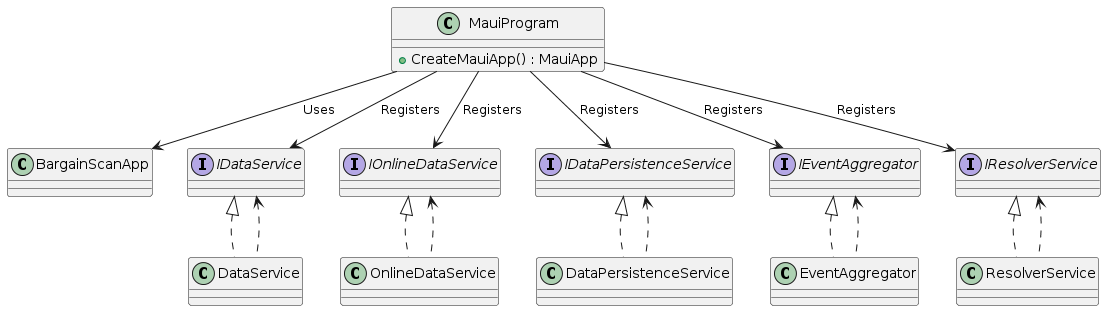
\includegraphics[width=1\linewidth]{img/app_services.png}
	\caption{Mobile App Services}
	\label{fig:appservices}
\end{figure}

Visible on figure \ref{fig:appservices}, the MauiProgram is the application's entry point, and it properly builds the BargainScanApp by injecting all of the required services into the dependency injection container. These services are required for the application to function properly while adhering to the key MVVM principles.

\noindent\textbf{ResolverService}

The ResolverService in automatically links Views to the ViewModels that go with them. It uses a naming convention where the ViewModel is called the same thing as the View, but with "Model" added at the end.

This service is registered with the dependency injection container, just like any other service. All classes that end in "View" or "ViewModel" are looked for in the app. It finds the ViewModel that goes with each View and registers a factory method that makes the View and sets its DataContext to a ViewModel instance.

With this method, setting the DataContext for a View is done automatically, so modules don't have to care for it. There is a separation of concerns with this approach, as Views are not connected to the creation and retrieval of their ViewModels.

\noindent\textbf{EventAggregator}

The EventAggregator is a communication mechanism that enables loosely coupled interactions between application components. It includes Publish, Subscribe, and UnSubscribe methods that allow components to communicate without using direct references.

In the MVVM pattern, the EventAggregator replaces standard .NET events to reduce coupling and improve modularity. It enables components to communicate without knowing each other, thereby increasing reusability and testability. This is especially important in MVVM, where separation of concerns and loose coupling are fundamental principles.

\noindent\textbf{OnlineDataService and DataPersistenceService}

It is the OnlineDataService's responsibility to communicate with the API; however, it is only used when the application lacks data or has outdated data about the products contained in the API. The DataPersistenceService is used to load and save retrieved shop items, the local user profile, the user's registered shopping carts, and descriptive information.

\noindent\textbf{DataService}

\begin{figure}[H]
	\centering
	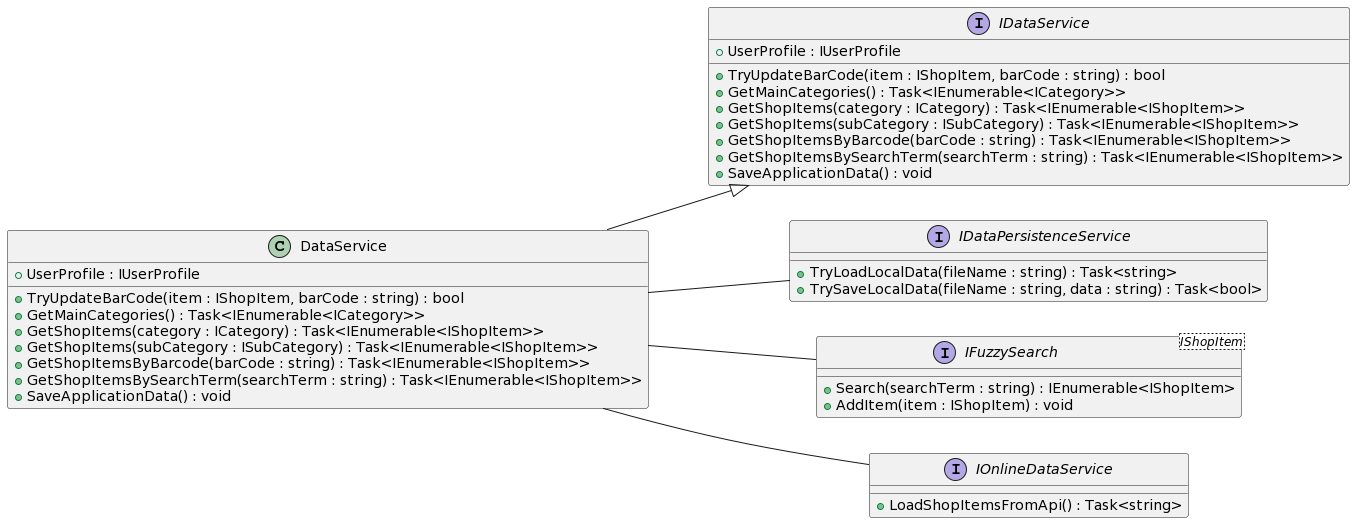
\includegraphics[width=1\linewidth]{img/app_dataservice.png}
	\caption{Mobile App DataService}
	\label{fig:appdataservice}
\end{figure}

The \textbf{DataService}, visible on figure \ref{fig:appdataservice}, is the primary service that allows users to access and manipulate application data across the entirety of the application. It makes use of IDataPersistenceService for the purpose of saving and loading local data, and it makes use of IOnlineDataService for the purpose of accessing data from the API. 

It is responsible for implementing the IDataService interface, which defines the methods that the service offers. Through the process of build-up, the service is injected into the application, which guarantees that it will be accessible throughout the entirety of the runtime. It is possible to execute the majority of the DataService's methods in an asynchronous manner, which guarantees that the user interface will not become unresponsive in situations where a lot of computational power is required. 

The modules that make use of it are able to access shop items classified into particular categories or subcategories, as well as search for those items using barcodes or search terms, with the latter method employing fuzzy string matching for improved performance. It also manages the process of assigning a barcode to a product in the event that the product has not yet been assigned with a barcode. 

\pagebreak

The service is also in charge of handling data for the local user profile, managing registered shopping carts, determining which shopping cart is active, and allowing the metadata and content of the shopping carts to be modified.

Additionally, it offers a method for saving application data on the fly, and it is responsible for loading information from either local or online sources when the application is started up. It is important to note that the data that is saved locally is saved in the data folder of the application using the JSON format. This ensures that the data is secure and invisible to any malicious attempts. 

\noindent\textbf{FuzzySearch}

As part of DataService a generic class called FuzzySearch is used to perform fuzzy searches on a group of objects of type T that implement the INamed interface. Similarity scores are computed using the Fuzz class from the FuzzySharp NuGet package.

The class keeps an index that is reversed for effective searching. The AddItem(T item) function creates n-grams from the item's name in order to add it to the index.

Fuzzy search is carried out by the Search(string searchTerm) method, which generates n-grams from the search term, retrieves matching items from the index, uses Fuzz's PartialRatio to calculate a score for each item, and returns items sorted by score if their score is higher than a threshold.

\begin{algorithm}
	\caption{Search Method}
	\begin{algorithmic}
		\State Initialize set $candidates$
		\For{each n-gram in GenerateNGrams($searchTerm$, 3)}
		\If{n-gram is in \_invertedIndex}
		\For{each item in \_invertedIndex[n-gram]}
		\State Add item to $candidates$
		\EndFor
		\EndIf
		\EndFor
		\State Initialize list $matchedItems$
		\For{each candidate in $candidates$}
		\State Calculate $score$ as Fuzz.PartialRatio of $searchTerm$ and candidate's name
		\If{$score$ is greater than ThresholdScore}
		\State Add candidate to $matchedItems$
		\EndIf
		\EndFor
		\State Sort $matchedItems$ by score in descending order
		\newline
		\Return $matchedItems$
	\end{algorithmic}
\end{algorithm}

\subsubsection{Model Layer}

Each and every significant data model that is required for data handling and manipulation is contained within the Model layer. 

The ShopItem, ShoppingCart, and UserProfile classes have been implemented in such a way that they contain JSON attributes for relevant properties. This ensures that the data is retrieved, saved, and loaded correctly. Additionally, it ensures that important information is not lost during the process of serializing and deserializing the data. 

In general, the models are implemented with properties and methods that adhere to naming conventions that make it simple to deduce the responsibilities and logic that lie behind them. Models that were utilized in the application are depicted in the figure that can be found on figure \ref{fig:appmodels} below.

\begin{figure}[H]
	\centering
	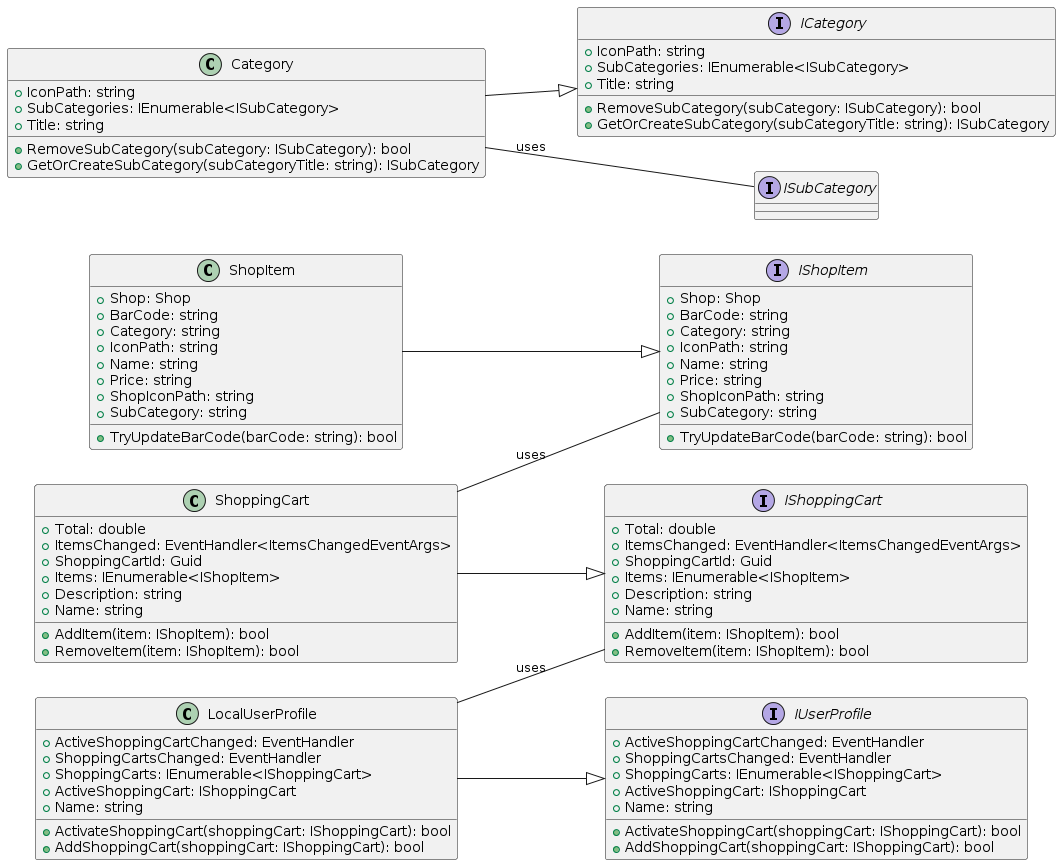
\includegraphics[width=1\linewidth]{img/app_models.png}
	\caption{Mobile App Models}
	\label{fig:appmodels}
\end{figure}

\subsubsection{Presentation Layer (View, ViewModel)}

Due to the fact that both the View and ViewModel layers are accountable for the configuration of the user interface, they are discussed together in this instance. 

The user interface of the application can be broken down into four primary sections: \begin{itemize}
	\item the shell, which provides a menu for navigating between categories;
	\item the main page, which is in charge of presenting the items for a particular category;
	\item the barcode page, which is in charge of scanning barcodes;
	\item  and the user profile page, which is responsible for accessing shopping carts.
\end{itemize} 
Additionally there's a popup for searching for items by their name.

Since the application is heavily dependent on the MVVM design pattern, the ViewModels implement INotifyPropertyChanged in order to update the View with information about changed properties. Additionally, the ViewModels implement the IHandle interface in order to handle messages that are published by the EventAggregator. The Views are being initialized and registered through the use of ResolverService, and I have avoided using the code-behind as much as possible, because doing so is also a violation of the pattern.

There are additional ViewModels which are not matched by their own Views. The reason behind this is that the models used in this case are not enough by themselves and need an extra layer of presentation logic to make sense for the user interface.

The general architecture of the layer can be seen on figure \ref{fig:appviewmodels} below.

\begin{figure}[H]
	\centering
	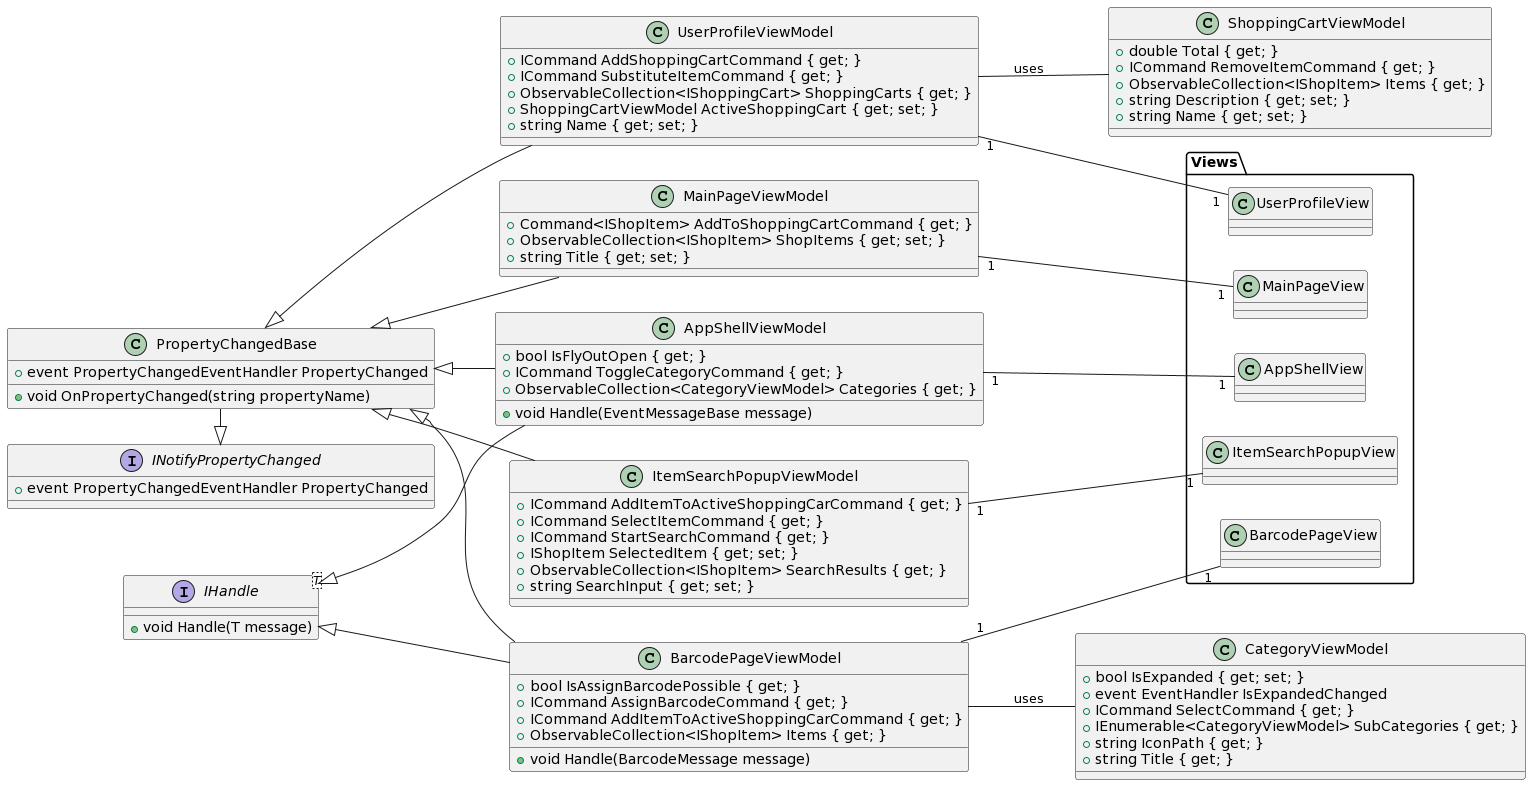
\includegraphics[width=1\linewidth]{img/app_viewmodels.png}
	\caption{Mobile App Views and ViewModels}
	\label{fig:appviewmodels}
\end{figure}

\noindent\textbf{Main page and Shell Fly-Out}

All of the items that fall under the chosen category are displayed on the main page. Every time a new category is chosen, the content is automatically updated in a dynamic manner. Each of these items displays the name of the store from which they originate and can be added to the shopping cart that is currently active. 

The flyout of the shell is utilized for the purpose of presenting the list of categories and subcategories that are available. The list of subcategories expands and shrinks depending on whether the main category is clicked on or not. 

The UI implementation is presented on figure \ref{fig:appitemspage} below.

\begin{figure}[H]
	\centering
	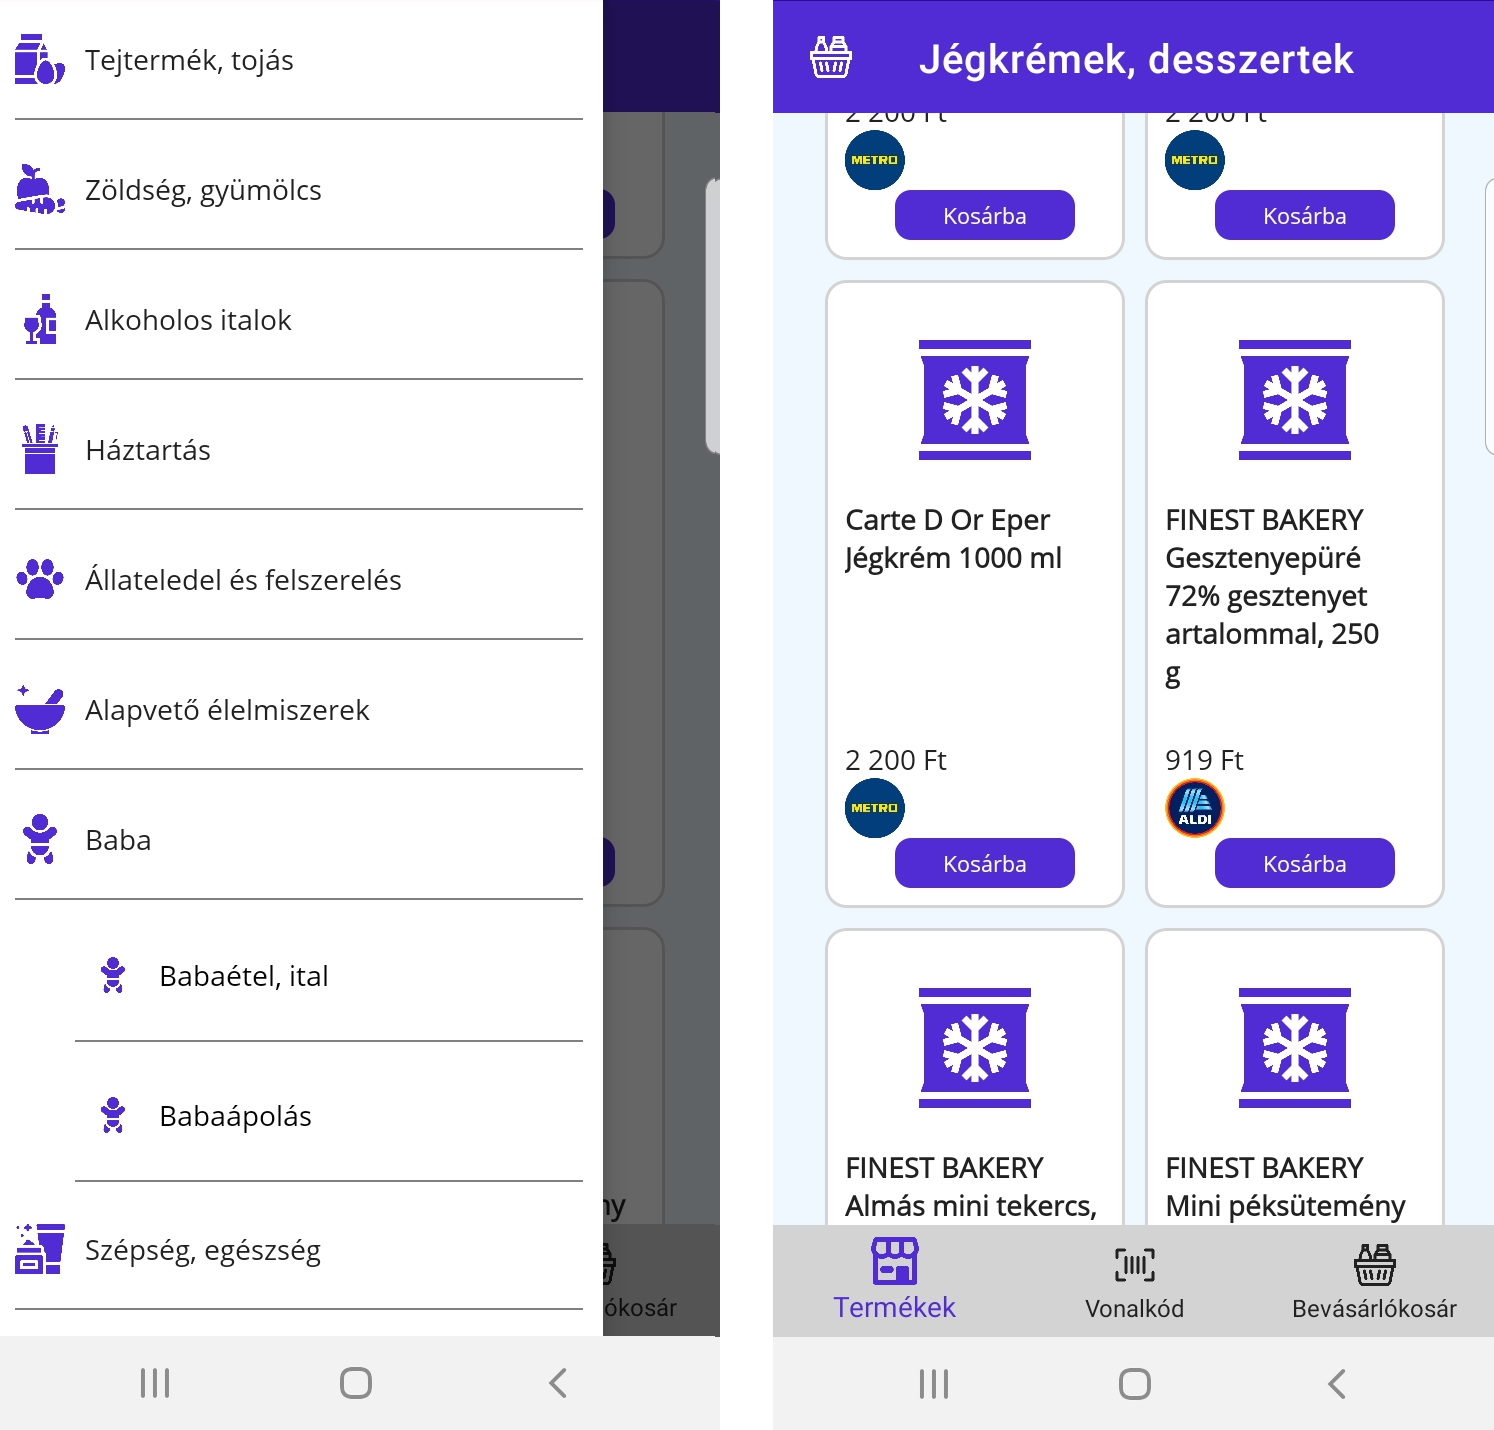
\includegraphics[width=0.5\linewidth]{img/app_itemspage.png}
	\caption{Mobile App Main Page and Shell Fly-out}
	\label{fig:appitemspage}
\end{figure}

\noindent\textbf{Barcode Page}

The barcode page includes a camera-view for reading item barcodes. After reading the code for an item, the app attempts to locate it in the repository. If it contains matching item(s), they are displayed and can be added to the current shopping cart. 

If no items match, the user can manually assign the code to any items that do not already have a code assigned. For this purpose, the search popup shown in figure \ref{fig:appsearchpopup} is used.

Figure \ref{fig:appbarcodepage} on the next page shows how the barcode page was implemented.

\begin{figure}[H]
	\centering
	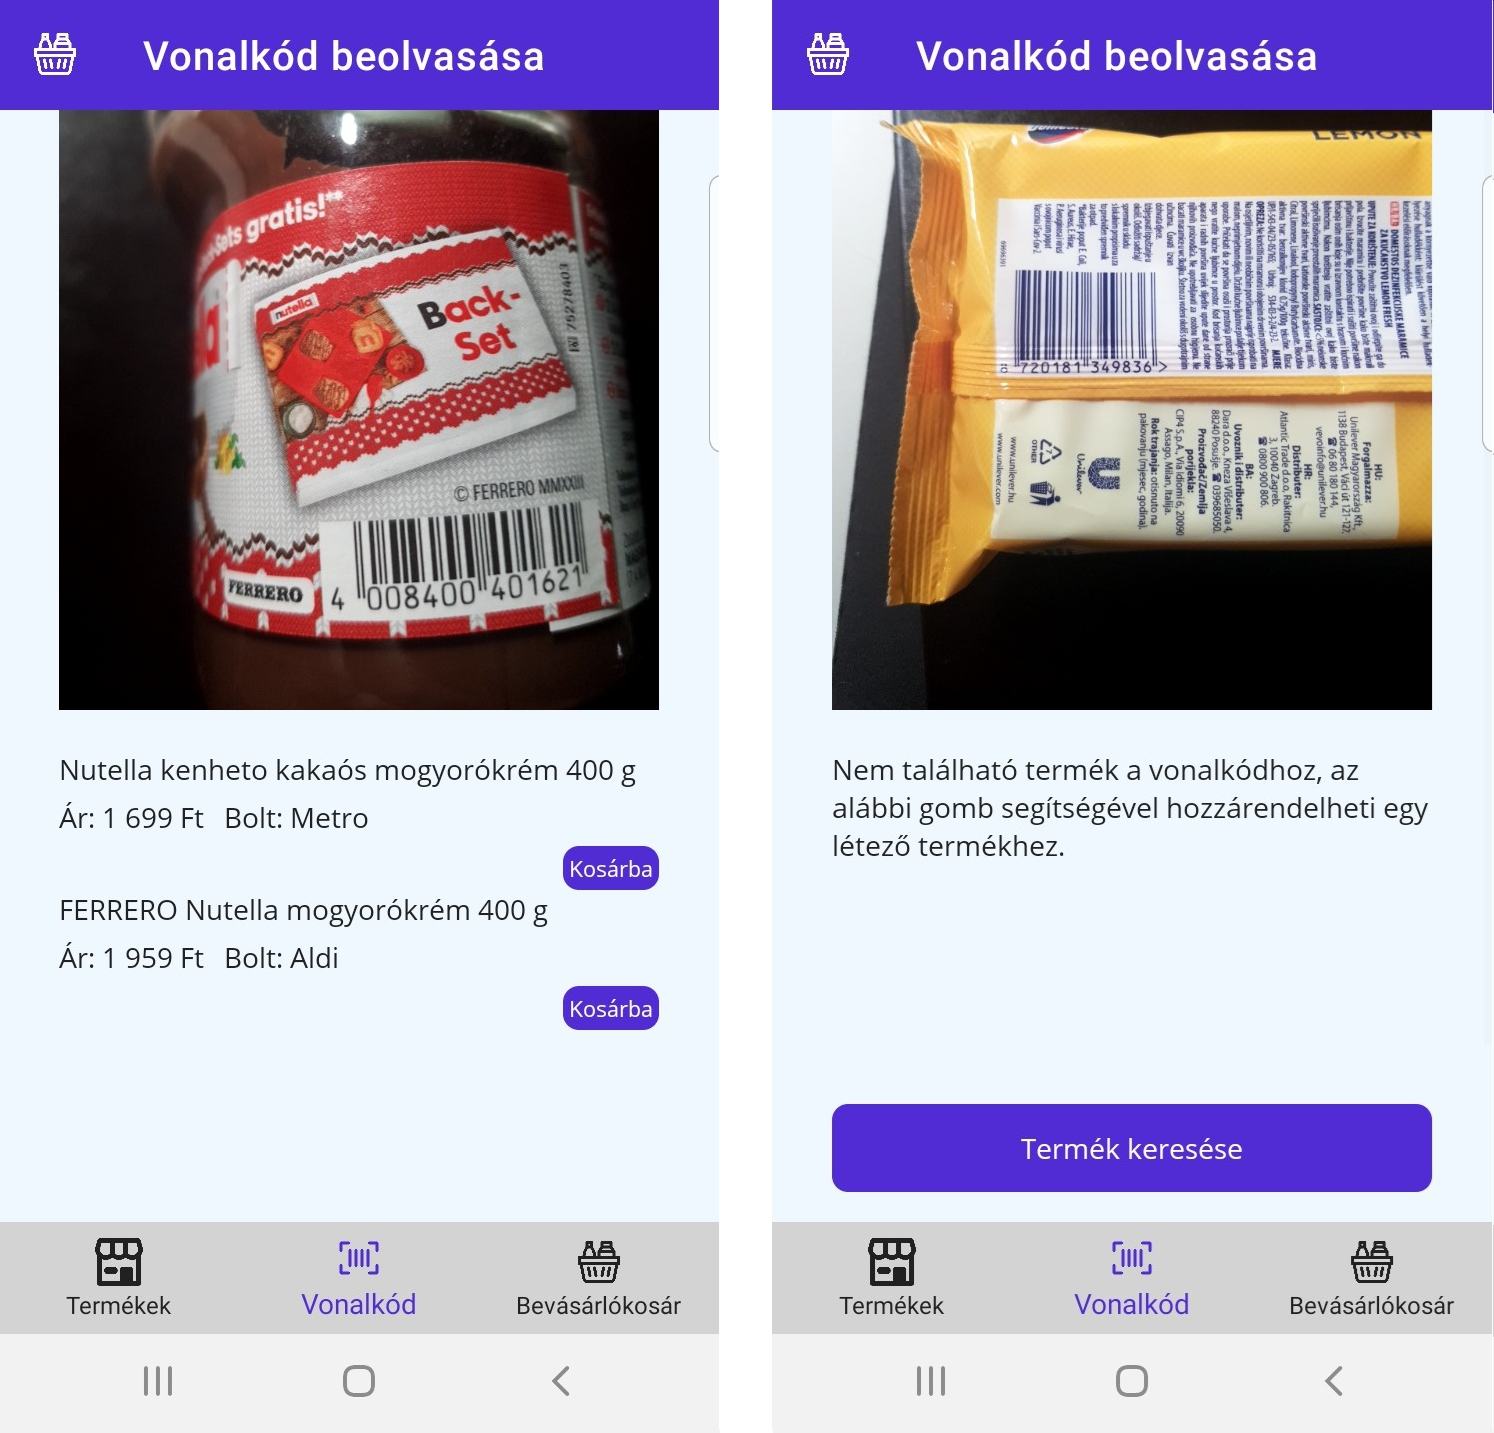
\includegraphics[width=0.6\linewidth]{img/app_barcodepage.png}
	\caption{Mobile App Barcode Page}
	\label{fig:appbarcodepage}
\end{figure}

\noindent\textbf{User profile / Shopping Carts Page}

\begin{figure}[H]
	\centering
	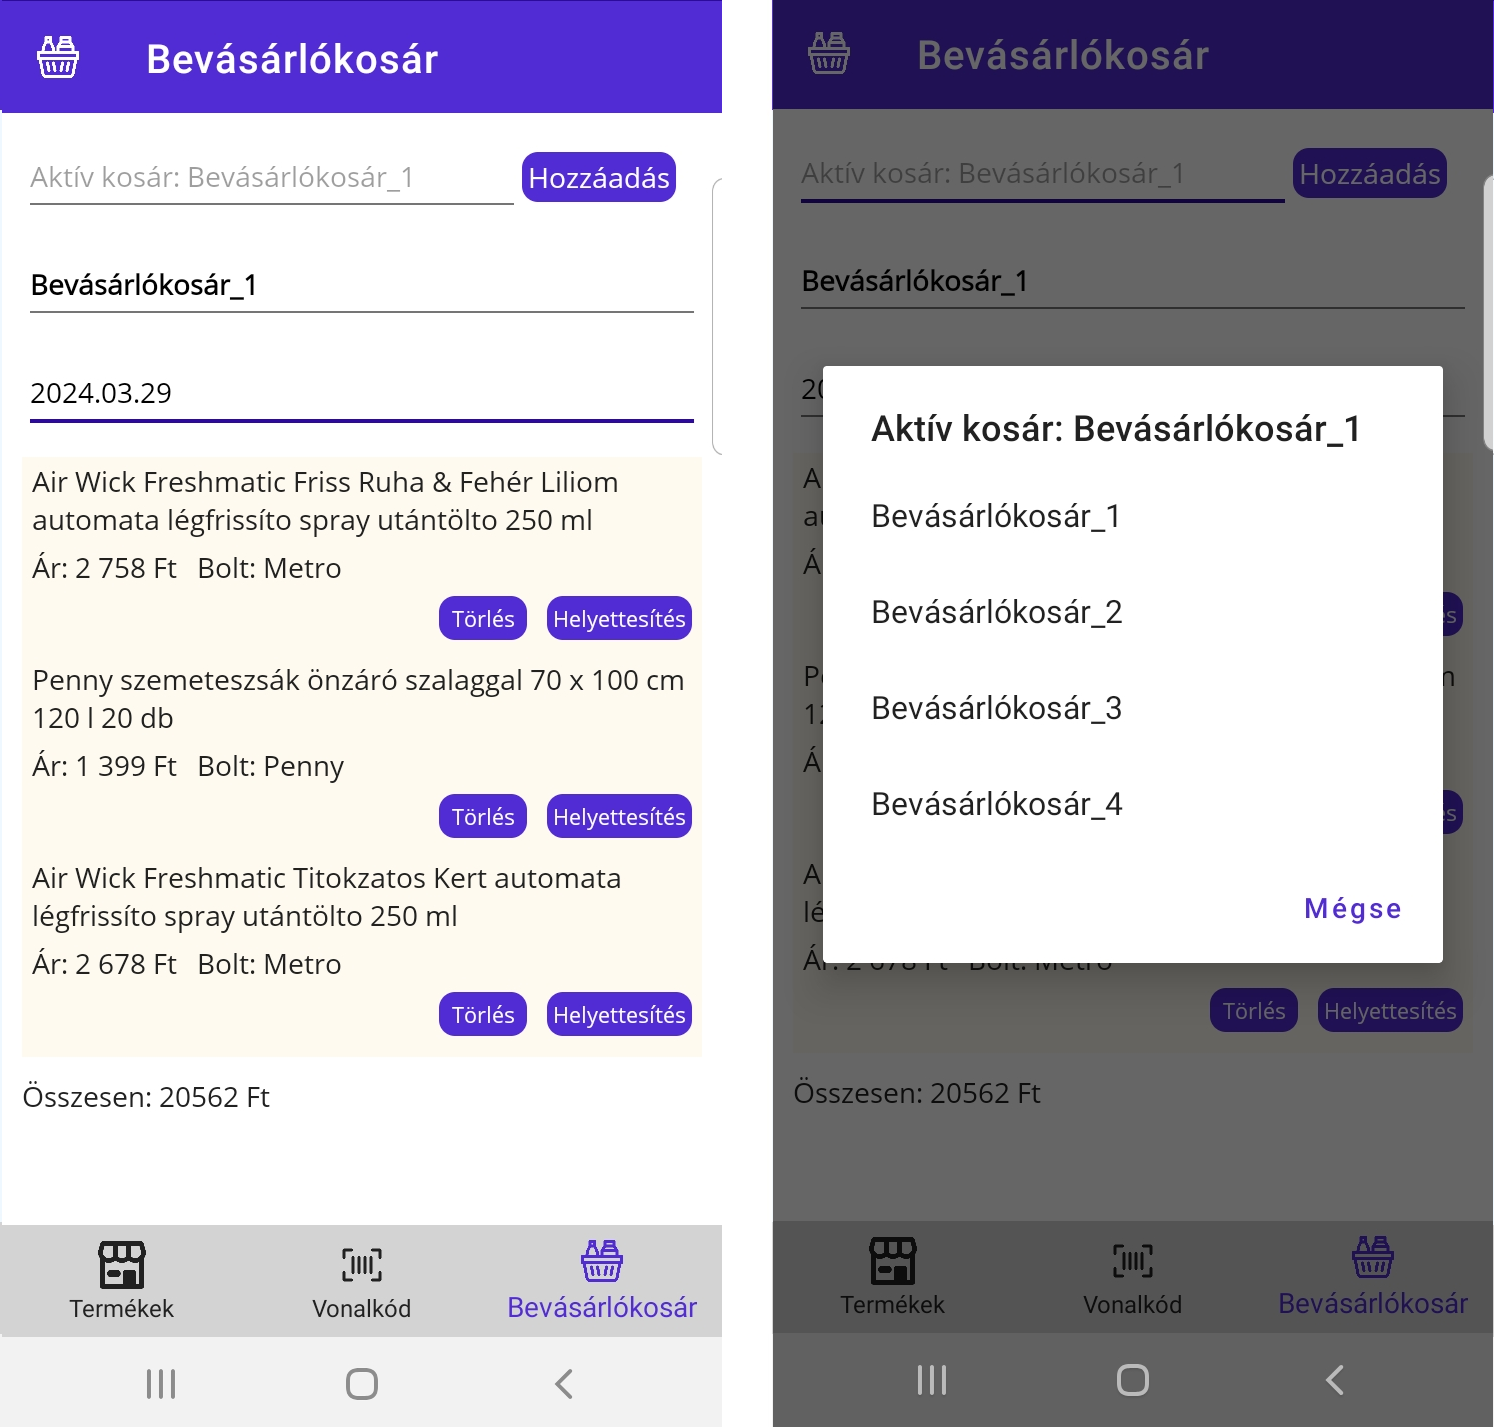
\includegraphics[width=0.6\linewidth]{img/app_shoppingcartpage.png}
	\caption{Mobile App User Profile Page}
	\label{fig:appshoppingcartspage}
\end{figure}

The way the presentation for the user profile and its associated shopping carts is implemented is visible on figure \ref{fig:appshoppingcartspage} above.

The page displays the active shopping cart and allows the user to switch between carts.  A scrollable popup allows users to switch between shopping carts. Selecting a shopping cart activates it. The shopping carts include metadata such as name and description. All shopping carts contain and store the items that the user adds to them. 

The shopping cart view shows the current items in the cart as well as the total number of items included; the user can also remove or substitute items. The substitution makes use of the previously mentioned item searching popup, as shown on figure \ref{fig:appsearchpopup}.

\noindent\textbf{Search Popup}

Finally, let's discuss the popup that allows the user to search for items stored in the repository. To return results, the search must contain at least three characters. If there are too many results, the user will be shown the top ten.  Scrolling through the popup reveals the hidden hits. 

The popup displays the select command for modules that use it. When an item is selected, the calling module receives the item's reference. It also includes a "Add to cart" command so that users can easily add items to their shopping cart if they discover something they forgot to add previously.

The realized user interface of the popup is visible on figure \ref{fig:appsearchpopup} below.

\begin{figure}[H]
	\centering
	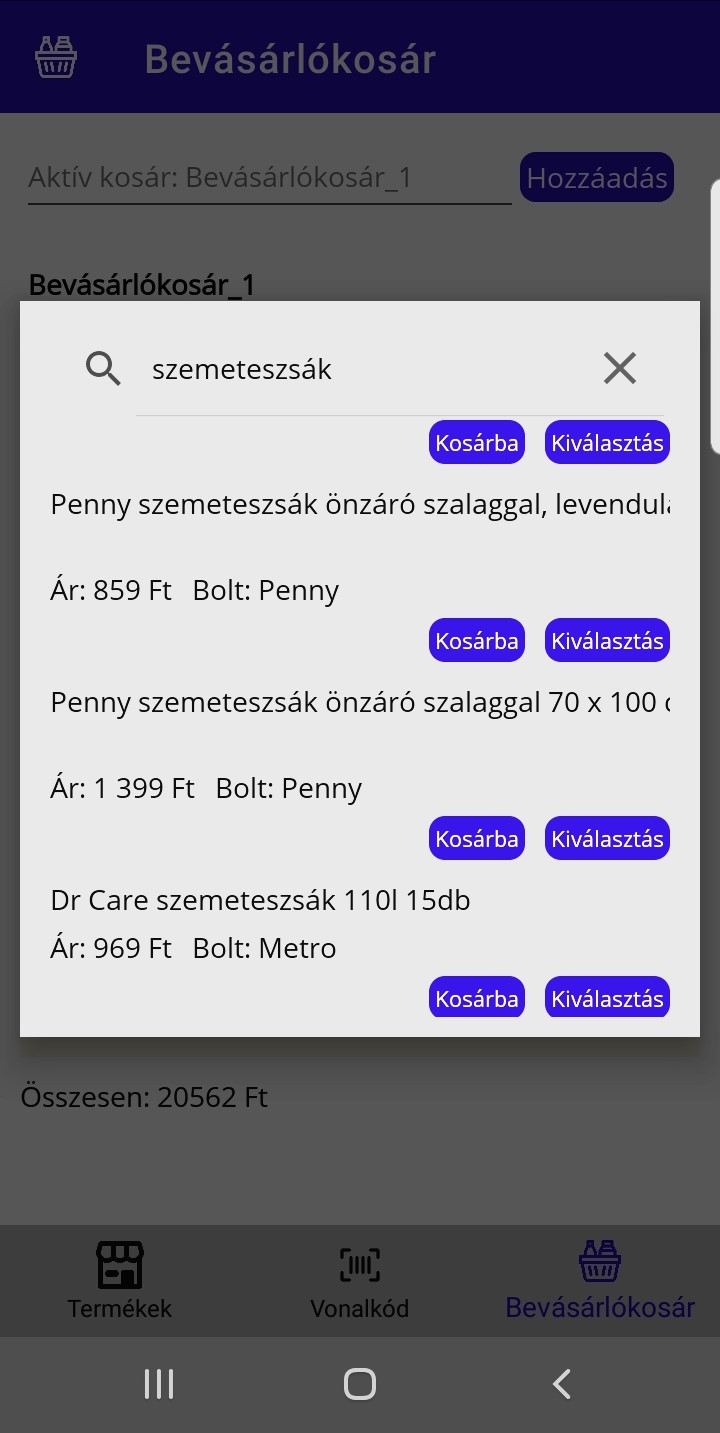
\includegraphics[width=0.3\linewidth]{img/app_search.png}
	\caption{Mobile App Search Popup}
	\label{fig:appsearchpopup}
\end{figure}

\clearpage
\section{TESTING}
\input{chapters/7_testing}

\clearpage
\section{CONCLUSION}
The project's scope, which was originally intended as a mobile application, has grown significantly due to web scraping, data collection, administration, and other features. This evolution necessitated the creation of a complete software solution that included an API, database, web application, and the mobile application. 

Given the expanded scope, it was necessary to use a Minimum Viable Product (MVP) approach. This strategic decision was motivated by the realization that developing all of the planned functionality would take longer than expected, and the solution would become obsolete before it was released. Thus, focusing on the MVP allowed me to prioritize core features that would provide immediate value while still leaving room for future development.

\noindent\textbf{Utilization of Current Technologies and Frameworks}

Despite its focus on MVP, the project does not make any compromises in terms of technology. Through the utilization of well-known and cutting-edge technologies and frameworks, such as Angular, MongoDB, ASP.NET and MAUI, the project guarantees that the product will continue to be robust, scalable, and in accordance with the most recent industry standards. These technologies offer a solid basis for future expansions and ensure that the product can adapt to changing user requirements and emerging trends, thus providing a reliable foundation for future expansions.

\noindent\textbf{Modular Design and Clean Coding Principles}

The modular architecture and use of clean coding standards were crucial for dealing with the complexity within a short time span. The modular structure enables for the isolation and development of functions individually, making the system easier to comprehend, test, and develop. Clean coding techniques guarantee that code is maintainable and self-explanatory, which is especially useful when projects are running on tight deadlines and future scalability is a worry. \cite{cleancode}

\noindent\textbf{Continuing Development}

The Agile methodology, with its adaptability and responsiveness, is ideal for the ongoing development of this comprehensive software solution. As the project progresses, agile practices will become increasingly important because they are incremental and iterative. This approach allows for continuous evaluation and integration of feedback, ensuring that all software components, including the API, database, web application, and mobile application, evolve in sync with user needs and technological advancements. \cite{agile}

\pagebreak

By implementing Agile, the project team can maintain flexibility and adjust the development path based on real-world testing and user feedback. This method is especially useful for dealing with the complexity and uncertainty of a multifaceted system design because it allows for frequent re-evaluation and refinement. As a result, Agile reduces the risk of deviating from user expectations or pursuing less impactful features, allowing each release to be as relevant and effective as possible. \cite{agile}

\noindent\textbf{Key Challenges and Future Directions}

One of the key issues faced throughout development was a scarcity of free barcode repositories, which caused a significant bottleneck. This constraint required manual barcode dispensing using cellphones, which proved cumbersome and inefficient. Addressing this issue before final release is important to progressing effectively. Identifying or inventing a simpler, more automated barcode system will be critical for improving user comfort and functionality.

\subsection{Future Prospects and Continuous Improvement}

Looking ahead, the MVP serves as an essential stage toward a more comprehensive system. The architecture's inherent flexibility and clean, modular design allow for the addition of new features and enhancements as time and user feedback permit. The initial ideas for future improvement are technology and infrastructure, user interface and accessibility, and strategic partnerships.

\noindent\textbf{Technology and Infrastructure}

\begin{itemize}
	\item \textbf{Local Database Integration:} Transitioning from storing local-data in a file-based manner to using a local database in the mobile application will be explored to improve the speed and reliability of data retrieval and storage.
	\item \textbf{Web Scraping Enhancements:} It is intended to employ Google's upcoming AI capabilities to enhance and simplify web scraping procedures. The purpose of this improvement is to enable more effective data extraction from online sources, resulting in increased responsiveness and accuracy.
	\item \textbf{iOS Expansion:} It is planned to enter the iOS market in order to broaden the scope of the audience that may be reached.
	\item \textbf{Pricing and Location-Based Algorithms:} Future objectives include developing a price-based calculation algorithm to assist users in selecting the most cost-effective shopping alternatives as well as implementing map-based shopping recommendations based on their location and interests.
\end{itemize}

\pagebreak

\noindent\textbf{User Interface and Accessibility}

\begin{itemize}
	\item \textbf{Online User Profile and Authentication:} Implementing an online user profile and authentication system on the mobile app protects user data, personalizes the experience, and allows for cross-device switching. The API already supports this feature.
	\item \textbf{Two-Tiered Application Model:} There are plans to provide both an ad-supported free version and a premium, ad-free edition, which may contain additional exclusive features for improved functionality and user experience.
\end{itemize}

\noindent\textbf{Strategic Partnerships}

These are crucial for tackling the most important issue regarding the lack of available free barcode repositories the application is facing.

\begin{itemize}
	\item \textbf{Partnerships with Retailers:} Plans include creating strategic alliances with businesses to gain access to their inventory of items and barcodes. This partnership makes it easier to add and accurately identify items inside the application, as well as improve the user experience by offering detailed product data.
	\item \textbf{Partnership with Barcode Repositories:} Collaboration with dedicated barcode storage facilities is also on the plan. This provides access to a diverse set of product barcodes, ensuring full coverage and up-to-date information across several product categories.
\end{itemize}

\noindent\textbf{Ending Note}

This project started as a fundamental mobile app and rapidly grew into a full-fledged software solution that incorporates web scraping, authentication, data management, and user interfaces for both web and mobile platforms. Because of the extensive scope and the need for rapid demonstrable results, MVP strategy was required. This strategy guaranteed that I only had to concentrate on fundamental functions, reducing the danger of outmoded technology before it even reached the market.

One important issue was a scarcity of free barcode containers, which necessitated tedious manual procedures. Addressing issue before the final release will be critical to improve the user experience and operational efficiency.

The MVP's foundations, coupled with its modular design and clean coding techniques, establish the platform for future advancements, allowing the project to adapt and expand in response to user input and developing demands.



% ------------------------------------------------------

% JEGYZÉKEK, INNEN KI LEHET KOMMENTEZNI AMELYIK ESETLEG NEM KELL (de ha van ábra/táblázat akkor kötelező, irodalomjegyzék kötelező, rövidítések opcionális)

\clearpage
\section{BIBLIOGRAPHY}
\printbibliography[heading=none]

\clearpage
\renewcommand{\listfigurename}{LIST OF FIGURES}
\listoffigures

\clearpage
\renewcommand{\listtablename}{LIST OF TABLES}
\listoftables

\clearpage

\end{document}
